%-------------------------------------------------------------------------------
%                      Template Naskah Skripsi
%               	Berdasarkan format JTETI FT UGM
% 						(c) @gunturdputra 2014
%-------------------------------------------------------------------------------

%Template pembuatan naskah skripsi.
\documentclass{jtetiskripsi}

%Untuk prefiks pada daftar gambar dan tabel
\usepackage[titles]{tocloft}
\renewcommand\cftfigpresnum{Gambar\  }
\renewcommand\cfttabpresnum{Tabel\   }

%Untuk hyperlink dan table of content
\usepackage[hidelinks]{hyperref}
\newlength{\mylenf}
\settowidth{\mylenf}{\cftfigpresnum}
\setlength{\cftfignumwidth}{\dimexpr\mylenf+2em}
\setlength{\cfttabnumwidth}{\dimexpr\mylenf+2em}

%Untuk Bold Face pada Keterangan Gambar
\usepackage[labelfont=bf]{caption}

%Untuk caption dan subcaption
\usepackage{caption}
\usepackage{subcaption}

%pdf
\usepackage{pdfpages}

%table
\usepackage{array}
\usepackage{longtable}
\newcolumntype{P}[1]{>{\centering\arraybackslash}p{#1}}
\usepackage{graphics}
\usepackage{wrapfig}

%bibliography
\usepackage[
  style=authoryear-icomp,
  maxcitenames=1,
  isbn=false,
  doi=false,
  url=false,
  autolang=other,
  hyperref=true,
  sortcites=true,
  bibwarn=true,
  firstinits=true,
  autolang=other,
]{biblatex}
\DefineBibliographyStrings{english}{%
  andothers = {dkk\adddot,\addspace},
}
\DeclareFieldFormat{citehyperref}{%
  \DeclareFieldAlias{bibhyperref}{noformat}% Avoid nested links
  \bibhyperref{#1}}

\DeclareFieldFormat{textcitehyperref}{%
  \DeclareFieldAlias{bibhyperref}{noformat}% Avoid nested links
  \bibhyperref{%
    #1%
    \ifbool{cbx:parens}
      {\bibcloseparen\global\boolfalse{cbx:parens}}
      {}}}

\savebibmacro{cite}
\savebibmacro{textcite}

\renewbibmacro*{cite}{%
  \printtext[citehyperref]{%
    \restorebibmacro{cite}%
    \usebibmacro{cite}}}

\renewbibmacro*{textcite}{%
  \ifboolexpr{
    ( not test {\iffieldundef{prenote}} and
      test {\ifnumequal{\value{citecount}}{1}} )
    or
    ( not test {\iffieldundef{postnote}} and
      test {\ifnumequal{\value{citecount}}{\value{citetotal}}} )
  }
    {\DeclareFieldAlias{textcitehyperref}{noformat}}
    {}%
  \printtext[textcitehyperref]{%
    \restorebibmacro{textcite}%
    \usebibmacro{textcite}}}
\addbibresource{daftar-pustaka.bib}
\renewbibmacro{in:}{}

%equation
\usepackage{amsmath}

%algorithm & syntax
\usepackage{algorithm}
\usepackage{algpseudocode}
\algnewcommand\algorithmicforeach{\textbf{for each:}}
\algnewcommand\ForEach{\item[ \algorithmicforeach]}
\algdef{SE}[DOWHILE]{Do}{doWhile}{\algorithmicdo}[1]{\algorithmicwhile\ #1}%
\newenvironment{conditions}
  {\par\vspace{\abovedisplayskip}\noindent\begin{tabular}{>{$}l<{$} @{${}={}$} l}}
  {\end{tabular}\par\vspace{\belowdisplayskip}}

%code
\usepackage{listings}
\usepackage{xcolor}
\definecolor{codegreen}{rgb}{0,0.6,0}
\definecolor{codegray}{rgb}{0.5,0.5,0.5}
\definecolor{codepurple}{rgb}{0.58,0,0.82}
\lstdefinestyle{mystyle}{
    commentstyle=\color{codegreen},
    keywordstyle=\color{magenta},
    numberstyle=\tiny\color{codegray},
    stringstyle=\color{codepurple},
    basicstyle=\ttfamily\footnotesize,
    frame=single,
    breakatwhitespace=false,
    breaklines=true,
    captionpos=b,
    keepspaces=true,
    numbersep=5pt,
    showspaces=false,
    showstringspaces=false,
    showtabs=false,
    tabsize=2
}
\lstset{style=mystyle}
\makeatletter
\def\thechapter{\@Roman\c@chapter}
\AtBeginDocument{%
  \def\thelstlisting{\@arabic\c@chapter.\@arabic\c@lstlisting}}
\makeatother


%-----------------------------------------------------------------
%Disini awal masukan untuk data proposal skripsi
%-----------------------------------------------------------------
\titleind{KLASIFIKASI IKAN MENGGUNAKAN VIOLA-JONES OBJECT DETECTION FRAMEWORK}

\fullname{Nehemiah Austen Pison}

\idnum{1313619021}

\approvaldate{8 Juni 2023}

\degree{Sarjana Ilmu Komputer}

\yearsubmit{2023}

\program{Ilmu Komputer}

\dept{Ilmu Komputer}

\firstsupervisor{Muhammad Eka Suryana, M. Kom.}
\firstnip{198512232012121002}

\secondsupervisor{Med Irzal, M. Kom.}
\secondnip{197706152003121001}

%-----------------------------------------------------------------
%Disini akhir masukan untuk data proposal skripsi
%-----------------------------------------------------------------

\tolerance=1
\emergencystretch=\maxdimen{}
\hyphenpenalty=10000
\hbadness=10000

\begin{document}

\cover{}
%-----------------------------------------------------------------

%-----------------------------------------------------------------
%Disini akhir masukan untuk muka skripsi
%-----------------------------------------------------------------

\chapter*{\centering{\large{LEMBAR PERSETUJUAN}}}
\thispagestyle{empty} {\bf }Dengan ini saya mahasiswa Fakultas
Matematika dan Ilmu Pengetahuan Alam, Universitas Negeri Jakarta

\vskip3mm

\begin{tabular}{ll}
  Nama & : Nehemiah Austen Pison \\
  No. Registrasi & : 1313619021 \\
  Program Studi & : Ilmu Komputer \\
  Judul & : Prototype System Klasifikasi Genus Ikan\\ & \hspace{0.2cm}
  Menggunakan Viola-Jones Feature Extraction\\ & \hspace{0.2cm}
  dan Boosting Berbasis Decision Tree
\end{tabular}

\vskip3mm

\noindent \hskip10mm Menyatakan bahwa proposal ini telah siap diajukan untuk seminar pra skripsi.
%\begin{center}
%Menyatakan bahwa skripsi ini telah siap diajukan untuk sidang skripsi.
%\end{center}



\begin{center}
\vskip3mm

Menyetujui,

\vskip3mm
\begin{spacing}{1.25}

\begin{tabular}{ccc}
  \hskip-2mm Dosen Pembimbing I & \qquad \qquad \qquad \qquad \qquad & \hskip-6mm Dosen Pembimbing II \\
   &  &  \\
   &  &  \\
   &  &  \\
   &  &  \\
  \hskip-2mm \underline{\textbf{Muhammad Eka Suryana, M.Kom}} &  & \hskip-6mm \underline{\textbf{Med
  Irzal, M.Kom}} \\
  \hskip-2mm NIP. 19770615 200312 1 001 &  & \hskip-6mm NIP. 19851223 201212 
  1 002	 \\
\end{tabular}
\end{spacing}
\end{center}
\vskip3mm
\begin{center}
Mengetahui, \\
Koordinator Program Studi Ilmu Komputer
\end{center}
\begin{spacing}{1.25}
{ \ }
\\
\\
{ \ }\begin{center}
\underline{\textbf{Dr. Ria Arafiyah, M.Si}} \\
{NIP. 19751121 200501 2 004}
\end{center}
\end{spacing} 

\chapter*{\centering{\large{KATA PENGANTAR}}}

Puji dan Syukur penulis panjakatkan kepada kehadirat Tuhan Yang Maha Esa, 
karena atas rahmat dan karunia-nya yang melimpah penulis dapat menyelesaikan
 skripsi ini dengan baik. Adapaun jenis penelitian dengan judul 
\textit{Prototype System Pendeteksi Spesies Ikan Menggunakan 
Viola-Jones Feature Extraction Dan Boosting Berbasis Decision Tree}.

Dalam menyelesaikan skripsi ini, penulis selalu mendapat bantuan dari orang 
di sekitar penulis baik dalam bentuk bimbingan dalam mengerjakan proposal 
ini maupun dorongan semangat dalam pengerjaan. Oleh maka dari itu, penulis 
ingin menyampaikan terima kasih yang sebesar-besarnya kepada:

\begin{enumerate}

	\item{Yth. Para petinggi di lingkungan FMIPA Universitas Negeri Jakarta}
	\item{Yth. Ibu Dr. Ria Arafiyah, M.Si selaku Koordinator Program Studi Ilmu
		Komputer.}
	\item{Yth. Bapak Muhammad Eka Suryana,M.Kom selaku Dosen Pembimbing I 
		yang telah membimbing dalam pengerjaan skripsi ini}
	\item{Yth. Bapak Med Irzal, M.Kom selaku Dosen Pembimbing II yang telah
		membimbing dalam pengerjaan skripsi ini.}
	\item{Orangtua penulis yang telah memberi dukungan selama pengerjaan
		 skripsi ini.}
	\item{Teman-teman yang telah memberikan dukungan dan bantuan dalam 
		pengerjaan skripsi ini.}
	
\end{enumerate}

Dalam penulisan skripsi ini penulis menyadari keterbatasan ilmu 
pengetahuan dan kemampuan penulis yang menyebabkan skripsi ini jauh dari 
sempurna, baik dari segi penulisan, penyajian materi, dan juga bahasa. Oleh 
karena itu penulis meminta kritik dan saran yang dapat djadikan sebagai 
pembelajaran serta dapat membangun penulis agar lebih baik lagi dalam mengerjakan 
tugas-tugas dan permasalahan yang ada kedepannya.

Akhir kata, penulis berharap skripsi ini dapat bermanfaat bagi semua 
pihak baik itu bagi FMIPA Universitas Negeri Jakarta, teman-teman dari progran 
studi Ilmu Komputer Universitas Negeri Jakarta dan para pembaca sekalian. 
Semoga Tuhan Yang Maha Esa senantiasa membalaskan kebaikan semua pihak yang 
telah membantu penulis dalam menyelesaikan skripsi ini.
\vspace{4cm}

\begin{tabular}{p{7.5cm}c}
	&Jakarta, 12 Januari 2024\\
	&\\
	&\\
	&\\
	&Nehemiah Austen Pison
\end{tabular}

%\singlespacing{}
\tableofcontents{}
\addcontentsline{toc}{chapter}{DAFTAR ISI}
\listoffigures{}
\addcontentsline{toc}{chapter}{DAFTAR GAMBAR}
\listoftables{}
\addcontentsline{toc}{chapter}{DAFTAR TABEL}

\begin{counterpage}
\end{counterpage}
%Disini awal masukan untuk Bab
%-----------------------------------------------------------------
%!TEX root = ./template-skripsi.tex
%-------------------------------------------------------------------------------
% 								BAB I
% 							LATAR BELAKANG
%-------------------------------------------------------------------------------

\chapter{PENDAHULUAN}

\section{Latar Belakang Masalah}

% Intro
Pasar ikan adalah sebuah pasar yang sangat besar, nilainya mencapai 
Rp. 2.400.000.000.000.000,- rupiah. Meskipun pasar yang besar, potensi 
perikanan di Indonesia belum maksmimal. 
Menurut Menteri Kelautan dan Perikanan RI Wahyu Sakti Trenggono, produktivitas 
perikanan di Indonesia masih kalah dari Vietnam (\cite{harianjogja}). 

% Sumber ikan
Ikan bisa didapatkan melalui dua sumber, dengan menangkap ikan dari habitat 
aslinya dan dengan melalukan proses pembudidayaan. Pembudidayaan ikan 
memerlukan banyak infrastruktur pendukung yang tidaklah murah seperti 
lahan, konstruksi tambak atau kolam yang memadai, dan pakan dalam jumlah 
yang cukup besar. Walaupun cukup mahal, budidaya ikan dapat 
menghasilkan keuntungan yang besar.  Ikan budidaya contohnya bisa dijual 
dalam keadan hidup atau segar ke wilayah-wilayah yang jauh dari habitat asli ikan, 
hal yang sulit dilakukan dengan ikan hasil tangkapan liar. Budidaya ikan 
juga dapat mengurangi permintaan pasar untuk ikan secara besar, yang secara tidak 
langsung berkontribusi terhadap berkurangnya \textit{overfishing} atau penangkapan 
ikan berlebih yang berdampak pada berkurangnya populasi ikan dalam jumlah 
yang besar di habitat aslinya. Permintaan untuk ikan sangat besar di 
Indonesia, hal ini menyebabkan besarnya nilai pasar dari industri ini. 
Kementrian Kelautan dan Perikanan Indonesia mencatat bahwa 
produksi ikan budidaya di Indonesia mencapai 14 juta ton pada tahun 
2021 dengan nilai sebesar Rp. 196.000.000.000.000,- rupiah (\cite{KKP}).

% Dasar problem permasalahan lapangan
Budidaya ikan di Indonesia memiliki problem yang lumayan besar yaitu 
diperlukannya usaha yang besar untuk menghitung dan mengawasi jumlah ikan 
yang dibudidayakan. Dalam penghitungan bibit pada proses jual beli contohnya, 
dalam menghitungan bibit lele para pedagang masih menghitung ikan dengan 
cara manual (\cite{alamri}). Bibit ikan dipindahkan satu persatu atau 
ditimbang sesuai berat untuk mendapatkan jumlah ikan. Cara-cara ini anatara sangat tidak 
efisien atau kurang akurat. Dalam metode penghitungan contohnya, ikan 
dihitung satu per satu dengan tangan atau dengan bantuan sendok atau centong, 
yang memungkinkan penghitung untuk mengambil ikan dengan jumlah tertentu. 
Metode ini bisa memakai waktu yang cukup lama bilamana ikan yang dihitung 
ada dalam jumlah besar, maka dari itu metode ini biasanya hanya digunakan 
dalam menghitung ikan dalam jumlah yang sedikit. Tingkat akurasi yang 
tinggi menjadi keuntungan utama dari metode penghitungan.

Sementara itu metode penimbangan hanya menghasilkan jumlah perkiraan yang tidak 
selalu akurat. Dalam metode ini bibit ikan dimasukan ke dalam suatu wadah dan lalu 
beratnya dihitung menggunakan timbangan. Berat hasil penimbangan lalu bisa 
dijadikan acuan kira-kira jumlah ikan yang terdapat di dalam wadah. 
Metode ini cepat dan cukup efisien dalam menghitung ikan dalam jumlah yang 
sangat besar. Namun jumlah bibit ikan tidaklah akurat dan hanya berupa perkiraan belaka.

% Elaborasi lebih lanjut problem lapangan
Problem perhitungan ikan ini akan sangat terasa pada industri budidaya ikan yang 
sangat mementingkan kepadatan populasi dalam tempat budidaya ikan. Populasi ikan 
yang berlebihan dapat memperlambat pertumbuhan ikan (\cite{diansarietal}), tapi 
di sisi lain populasi ikan yang terlalu kecil akan mengurangi efisiensi lahan 
yang dimiliki peternak ikan. Dalam mengatasi problem \cite{alamri} menciptakan 
sebuah sistem penghitungan menggunakan sensor \emph{proximity}. Hasil uji coba mendapat 
hasil yang baik dengan persentase error sebesar 4,07\% dengan penghitungan 
memakan waktu 228 detik per 1000 ikan. Jauh lebih cepat dibanding kecepatan 
hitung manual yang memakan waktu 20 menit per 1000 ikan. Cara lain dipakai 
oleh \cite{rusydi} untuk mendeteksi ikan. Rusydi menciptakan sebuah alat 
penghitungan dengan katup otomatis yang akan terbuka bilamana jumlah ikan 
yang diinginkan telah tercapai. Alat tersebut mendeteksi ikan menggunakan 
konsep \emph{through beam} di mana ikan akan terdeteksi ketika melewati pipa oleh 
inframerah dan photodioda. Alat tersebut dapat mendeteksi ikan dengan 
kecepatan 58 ms per ikan dengan tingkat akurasi 100\%.

% Kelemahan metode penghitungan manual Al-Amri dan Rusydi
Penggunaan alat deteksi fisik seperti yang digunakan \cite{alamri} maupun 
\cite{rusydi} memiliki beberapa kekurangan, seperti ukuran ikan bergantung 
kepada ukuran alat yang dipergunakan. Alat Rusydi sangat bergantung 
dengan kelandaian dan kecepatan lewat ikan yang melewati pipa sensor, mengganti 
ukuran ikan yang akan dideteksi mengharuskan tes ulang untuk 
mendapatkan pengaturan alat yang paling optimal (dalam tes, Rusyidi 
menemukan bahwa kelandaian pipa 30° memberikan hasil paling akurat dalam 
mendeteksi ikan). Sementara pada alat Al-Amri, lubang keluar 
ikan yang perlu dimodifikasi untuk mengamodasi ikan yang lebih besar. 
Metode-metode tersebut sangatlah tidak fleksibel dalam industri peternakan 
ikan yang tidak hanya menternakan satu jenis ikan saja.

% Penjelasan Rapid Object Detection
Deteksi Objek Cepat (\emph{Rapid Object Detection}) adalah sebuah algoritma yang 
diciptakan untuk pendeteksian muka \cite{violaetal}. Viola 
menjelaskan kalau algoritma deteksi yang diciptakannya dapat mendeteksi 
muka dari gambar berukuran 384 x 288 pixel dari kamera berkecepatan 15 
\textit{frame} per detik. Deteksi objek dapat digunakan untuk berbagai hal seperti 
anotasi gambar, penghitungan mobil, deteksi muka, rekognisi muka, pelacakan 
gambar dan lain-lain. Setiap algoritma deteksi objek bekerja dengan cara yang 
berbeda-beda namun dengan konsep yang kurang lebih sama. Setiap kelas objek 
pasti memiliki fitur yang dapat menunjukan jati diri objek tersebut, misalnya 
objek bola sepak pastilah bulat dan umumnya memiliki dua warna yaitu hitam dan 
putih dengan pola yang spesifik. Muka manusia memiliki mata, hidung dan mulut 
yang dapat dibedakan dengan mahluk lainnya misalnya dengan kucing. Metode-metode 
deteksi objek umumnya menggunakan pendekatan neural network dan 
\textit{non-neural network} untuk mendefinisikan fitur dari kelas objek yang 
berusaha dideteksi.

% Metode Adaboost
Adaboost (\cite{freundetal}) adalah sebuah pendekatan \textit{non-neural network} 
yang sering digunakan untuk mendefinisikan fitur dari objek yang ingin 
dideteksi (\cite{weber}). Adaboost telah digunakan untuk deteksi berbagai objek 
seperti deteksi plat nomor kendaraan bermotor (\cite{hoetal}), deteksi muka 
(\cite{violaetal}), deteksi pesawat terbang (\cite{freundetal}) dan lain-lain. 
Adaboost mencari fitur sebuah kelas objek dengan menggunakan sekumpulan 
\emph{weak learner} untuk membuat sebuah \emph{strong learner}. 
Kumpulan weak learner tersebut nantinya akan dinilai sesuai dengan akurasi 
mereka, di mana weak learner yang secara konsisten benar menebak fitur sebuah 
objek akan memiliki nilai lebih dalam keputusan klasifikasi akhir. Freund 
menjelaskan bahwa metode Adaboost dapat digambarkan selayaknya seorang pejudi 
pacuan kuda yang kalah terus menerus. Pejudi tersebut lalu memutuskan untuk 
menjadikan teman-teman penjudinya menjadi acuan untuk taruhan berikutnya. 
Adaboost bekerja layaknya penjudi tersebut, membuat asumsi dari berbagai 
pendapat lemah. Tentu saja bilamana sang penjudi melihat bahwa seorang 
temannya bertaruh dengan baik berulang-ulang kali, maka dia akan 
memandang tinggi pendapatnya di atas teman-teman lainnya yang tidak menang 
sebanyak orang tersebut. Adaboost juga bekerja mirip dengan situasi tersebut.

% Usulan
Berdasarkan latar yang telah dijelaskan, penulis mengusulkan untuk mendeteksi 
jenis ikan dengan menggunakan metode \emph{Viola-Jones Object Detection Framework}. 
Adaboost dalam \emph{Viola-Jones Object Detection Framework} berguna untuk 
mengkonstruksi sebuah \emph{classifier} objek ikan yang nantinya dapat mendeteksi 
ikan dalam input gambar maupun video. Hasil yang diharapkan adalah sistem 
mampu mengklasifikasi ikan dari gambar maupun video secara akurat.

\section{Rumusan Masalah}
Dari uraian permasalahan di atas, perumusan masalah dalam penelitian ini adalah 
'\textbf{Bagaimana cara mengklasifikasi ikan menggunakan metode 
\textit{Viola-Jones Object Detection Framework}?}'.

\section{Batasan Masalah}
Batasan masalah pada penelitian ini adalah:
\begin{enumerate}
	\item Klasifikasi ikan menggunakan \textit{Viola-Jones Object Detection Framework} yang didapat dari penelitian Viola-Jones (\cite{violaetal})
	\item Program didesain untuk mengklasifikasi ikan saja
	\item Klasifikasi dilakukan dengan gambar tampak samping ikan saja
	\item Klasifikasi harus bisa melakukan deteksi tiga kelas genus ikan, Abudefduf, Amphiprion, Chaetodon, 
	dan satu kelas negatif.
\end{enumerate}

\section{Tujuan Penelitian}
	Tujuan dari penelitian ini adalah menciptakan metode yang mampu mempermudah 
	klasifikasi ikan dengan menggunakan \textit{Viola-Jones Object Detection Framework}.

\section{Manfaat Penelitian}
\begin{enumerate}
	\item Bagi penulis
		
	Memperoleh gelar sarjana dalam bidang Ilmu Komputer, serta menambahkan 
	pengalaman dalam pembuatan sebuah program komputer dengan aplikasi dunia 
	nyata. Dan menambahkan pengetahuan penulis tentang deteksi objek, metode 
	\textit{Adaboost} dan \textit{Harr-Like Features}.
		
	\item Bagi Program Studi Ilmu Komputer
	
	\begin{itemize}
		\item Mahasiswa
		
		Diharapkan penelitian ini dapat digunakan sebagai penunjang referensi, 
		khususnya pustaka tentang klasifikasi object dengan 
		\textit{Viola-Jones Object Detection Framework}.

		\item Bagi Peneliti Selanjutnya
		
		Diharapkan penelitian ini dapat digunakan sebagai dasar atau kajian 
		awal bagi peneliti lain yang ingin meneliti permasalahan yang sama.

	\end{itemize}
			
\end{enumerate}

% Baris ini digunakan untuk membantu dalam melakukan sitasi
% Karena diapit dengan comment, maka baris ini akan diabaikan
% oleh compiler LaTeX.
\begin{comment}
\bibliography{daftar-pustaka}
\end{comment}

%!TEX root = ./template-skripsi.tex
%-------------------------------------------------------------------------------
%                            BAB II
%               KAJIAN TEORI
%-------------------------------------------------------------------------------

\chapter{KAJIAN PUSTAKA}

\section{Pengertian Klasifikasi Objek}

Fungsi dari klasifikasi objek adalah untuk memberikan deskripsi label ke 
sebuah segmentasi objek. Bila dilihat dari representasi fitur objek, ini 
dapat dicapai dengan melihat tanda-tanda keberadaan fitur yang mengindikasikan 
kelas dari objek. Hal ini umumnya dicapai dengan menentukan \textit{threshold} diantara 
kelas-kelas yang direpresentasikan oleh \textit{training set} yang sudah dilabeli. 
 Pelatihan otomatis umumnya mementingkan distribusi dari 
setiap kelas (distribusi harus setara), dan melabeli setiap contoh dengan benar, 
Namun, isu yang umum didalam cara ini pemilihan fitur-fitur yang akan digunakan untuk 
klasifikasi objek kadang kurang sesuai dan sering kali bergantung terhadap 
keberuntungan untuk mendapat hasil sangat akurat (\cite{rennoetal}).

\section{\emph{Viola Jones Object Detection Framework}}

Paul Viola dan Michael, J, Jones (\cite{rennoetal}) mempublikasikan sebuah makalah ilmiah dengan 
judul “\emph{Robust Real-Time Face Detection}”. Makalah tersebut mendeskripsikan sebuah 
framework pendeteksian wajah yang dapat memproses gambar secara cepat dengan 
tingkat akurasi yang tinggi. Ada tiga kontribusi penting dari makalah tersebut: 
Pertama adalah pengenalan sebuah representasi gambar baru yang dipanggil 
\emph{Integral Image} yang memungkinkan penghitungan fitur yang dipakai oleh detektor 
dilakukan dengan cepat. Yang kedua adalah sebuah classifier yang efisien dan 
sederhana, yang dibuat menggunakan algoritma pembelajaran \emph{Adaboost} 
(\cite{freundetal}) untuk memilih sejumlah fitur-fitur kritis dari 
fitur-fitur potensial. Yang ketiga adalah sebuah metode untuk menggabungkan 
fitur-fitur tersebut dalam sebuah bentuk \emph{cascade} yang memungkinakan algoritma 
untuk memfokuskan deteksi di area-area yang memiliki potensial saja.

\subsection{\emph{Features}}

\begin{figure}[H]
  \centering{}
	\includegraphics[width=0.6\textwidth]{gambar/haar\_features}
  \caption{Beberapa \emph{Haar-like features} yang digunakan framework Viola-Jones.}
\end{figure}

Ada banyak alasan dimana penggunaan fitur lebih baik daripada 
nilai piksel secara langsung. Alasan paling umum adalah fitur dapat berfungsi
untuk meng-\emph{encode ad-hoc domain knowledge} yang sulit dipelajari 
dengan jumlah data pelatihan yang terbatas. Untuk sistem \emph{framework Viola-Jones} 
ada alasan besar lainnya untuk penggunaan fitur yaitu sistem berbasis fitur beroperasi lebih cepat
daripada sistem yang berbasis nilai piksel.

Fitur sederhana yang digunakan mirip dengan \emph{Haar Basis Function} yang 
digunakan \cite{papaetal}. Lebih tepatnya ada tiga jenis fitur: dua persegi, tiga persegi dan 
empat persegi diagonal. 
Nilai dari sebuah \emph{fitur dua persegi} adalah perbedaaan diantara 
jumlah nilai piksel didalam dua atau lebih area persegi. Area-area tersebut memiliki 
ukuran dan bentuk yang sama, dan juga bersebelahan secara horizontal dan vertikal.
Subuah \emph{fitur tiga persegi} menghitung jumlah piksel dua area persegi 
di bagian luar dikurangi dengan jumlah nilai piksel persegi yang ada ditengah keduanya. 
Yang terakhir \emph{fitur empat persegi} menghitung perbedaan nilai dari dua pasang 
persegi diagonal.

% \subsection{\emph{Integral Image}}

% \begin{figure}[H]
%   \centering{}
% 	\includegraphics[width=0.6\textwidth]{gambar/integral\_image\_1}
%   \caption{Sebuah nilai \emph{Integral Image} $(x,y)$ dan area yang diwakilinyak}
% \end{figure}

% Fitur-fitur persegi dapat dihitung secara cepat menggunakan 
% representasi tidak langsung dari gambar, hal ini diberi nama 
% \emph{integral image}. \emph{integral image} pada lokasi $x, y$ berisikan 
% penjumlahan di atas dan di kiri dari $x, y$ dan nilai $x, y$ itu sendiri:
% \begin{equation}
%   i i(x, y)=\sum_{x^{\prime} \leq x, y^{\prime} \leq y} i\left(x^{\prime}, y^{\prime}\right),
% \end{equation}
% Dimana $ii(x,y)$ adalah \emph{integral image} dan $i(x,y)$ 
% adalah nilai piksel dari gambar aslinya. Menggunakan kedua 
% pengulangan berikut ini:
% \begin{equation}
%   s(x, y)=s(x, y-1) + i(x, y)
% \end{equation}
% \begin{equation}
%   ii(x, y)=ii(x-1, y) + s(x, y)
% \end{equation}
% (Dimana \emph{s(x, y)} adalah nilai kumulatif dari baris, \emph{s(x, -1) = 0}, 
% dan \emph{ii(-1, y) = 0}) \emph{Integral Image} dari sebuah gambar dapat dihitung dalam sekali jalan.

% \begin{figure}[H]
%   \centering{}
% 	\includegraphics[width=0.6\textwidth]{gambar/integral\_image\_2}
%   \caption{Jumlah dari intensitas cahaya pada persegi D dapat dihitung dengan 4 referensi \textit{array}. Nilai dari 1 adalah jumlah intensitas cahaya pada persegi A, Nilai dari 2 adalah persegi A + B, nilai dari 3 adalah A + C dan nilai 4 adalah A + B + C + D.}
% \end{figure}

% Menggunakan \emph{integral image}, semua jumlah nilai pada persegi dapat 
% dihitung didalam 4 referensi \emph{array}. Jelas perbedaan 
% diantara kedua jumlah nilai-nilai persegi dapat dihitung 
% dengan delapan referensi. Karena peresegi dua fitur yang 
% didefinisikan diatas melibatkan juga nilai persegi disebelahnya, 
% mereka dapat dikomputasi dengan enam referensi \emph{array}, delapan referensi
% bilamana ia adalah persegi tiga fitur, dan sembilan referensi untuk 
% persegi empat fitur.

% Kecepatan yang didapat dari penghitungan \emph{Integral Image} ini dapat dijustifikasi 
% bila kita membandingkannya dengan perhitungan manual. Sebagai contoh, misalkan 
% kita sedang mencari jumlah total intensitas cahaya pada ukuran area 10x10 
% piksel. Cara manual mengharuskan kita menghitung sampai 100 kali untuk mendapat 
% jumlah intensitas cahaya pada area tersebut, belum lagi proses ini harus 
% diulang terus-menerus untuk ukuran dan lokasi yang berbeda. Dilain sisi, 
% perhitungan menggunakan \emph{Integral Image} hanya perlu mereferensi tabel yang 
% sudah dibuat sebelum semua usaha klasifikasi, dalam hal ini kita hanya perlu 
% melakukan perhitungan empat kali untuk menghitung intensitas cahaya dalam area 
% tersebut.

\subsection{\emph{Adaboost}}

\begin{algorithm}
  \caption{Algoritma Adaboost}
  \begin{algorithmic}[1]
    \State Diberikan contoh gambar $(x_1, y_1), \ldots, (x_n, y_n)$ dimana 
    $y_i = 0$ untuk contoh negatif dan $y_i = 1, \ldots, N$ untuk contoh kelas-kelas positif
    \State Inisialisasi bobot $w_{i,1} = \frac{1}{\text{{total contoh}}}$
    \State Untuk $t = 1, \ldots, T$:
    \begin{enumerate}
      \item Normalisasi bobot, $w_{t,1} \gets \frac{w_{t,1}}{\sum_{j=1}^{n} w_{t,j}}$
      \item Pilih \textit{weak classifier} terbaik dengan melihat error yang telah diberi bobot
      \begin{equation}
        \in_t = \min_{f, p, \theta} \sum_i w_i |h(x_i, f, p, \theta) - y_i|.
      \end{equation}
      \item Definisikan $h_t(x) = h(x, f_t, p_t, \theta_t)$ dimana $f_t, p_t,$ dan $\theta_t$ adalah \textit{minimizer} dari $\in_t$.
      \item Perbarui bobot:
      \begin{equation}
        w_{t+1,i} = w_{t,i} \beta_t^{1 - e_i}
      \end{equation}
      dimana $e_i = 0$ bila contoh $x_i$ diklasifikasi secara benar, selainnya $e_i = 1$, dan $\beta_t = \frac{\in_t}{1 - \in_t}$
    \end{enumerate}
    \State \textit{strong classifier} akhirnya adalah:
    \begin{equation}
      C(x) = \begin{cases}
        1 & \sum_{t=1}^T \alpha_t h_t (x) \geq \frac{1}{2} \sum_{t=1}^T \alpha_t \\
        0 & \text{selain itu}
      \end{cases}
    \end{equation}
    dimana $\alpha_t = \log \frac{1}{\beta_t}$ 
  \end{algorithmic}
\end{algorithm}

Dalam \emph{framework Viola-Jones} sebuah varian dari \emph{Adaboost} 
digunakan untuk memilih fitur dan juga untuk melatih \textit{classifier}. 
Didalam bentuk aslinya, algoritma pembelajaran \emph{Adaboost} digunakan 
untuk mem-\textit{boost} performa klasifikasi dari algoritma pembelajaran 
sederhana. \emph{Adaboost} melakukan ini dengan menggabungkan sekumpulan 
\emph{classifier} lemah untuk membuat sebuah \emph{classifier} kuat. 
Didalam istilah \emph{Boosting}, \emph{classifier} lemah disebut juga 
dengan \emph{weak learner}. Sebagai contoh, algoritma pembelajaran \emph{perceptron} 
mencari dari sekelompok \emph{perceptron} dan mengambil \emph{perceptron} 
dengan tingkat kesalahan klasifikasi terendah. Algoritma pembelajaran disebut 
lemah karena kita tidak berharap \emph{classifier} terbaik untuk mengklasifikasi 
data dengan benar. Nyatanya, \emph{perceptron} terbaik mungkin 
hanya memiliki tingkat akurasi 51\%. Agar \emph{weak learner} dapat di-\textit{boost}, 
ia akan dipanggil untuk menyelesaikan sederet problem pembelajaran. Setelah 
satu ronde pembelajaran selesai, setiap contoh pembelajarannya akan dibobot ulang 
untuk menekankan problem yang salah diklasifikasi oleh \emph{weak learner} 
sebelumnya. Bentuk \emph{final strong classifier} adalah 
sebuah kombinasi \emph{weak learner} berbobot. 

\subsection{\emph{Weaklearn}}

\begin{algorithm}
  \caption{Metode Pembuatan \textit{Decision Tree}}
  \begin{algorithmic} [1]
    \State Anotasi semua dataset sesuai kelasnya. \textit{Decision Tree} lalu 
    akan dimulai dari akar
    \State Pilih atribut terbaik untuk melakukan \textit{split} dengan melakukan 
    \emph{Information Gain} (IG):
    \begin{equation}
      IG(S, A) = Entropi(S) - sum_v \frac{S_v}{S} x Entropi(S_v)
    \end{equation} 
    dimana:
    \begin{itemize}
      \item $S$: kumpulan sampel pada \emph{node} sekarang
      \item $A$: atribut yang digunakan untuk \textit{split}
      \item $v$: Sebuah nilai atribut $A$ yang membagi $S$ menjadi turunan $S_v$
      \item Entropi($S$) = $-sum_c p_c log_2(p_c)$: Ukuran kemurnian pada kumpulan 
      contoh dengan target label. Dimana $p_c$ adalah proporsi contoh $S$ yang ada 
      pada kelas $c$. 
    \end{itemize}
    %Masukin IGR kalo perlu (Information Gain Ratio)
    \State \textit{split} pohon ke \textit{node} turunan sesuai atribut yang dipilih 
    \State tentukan apabila seluruh contoh sudah jatuh ke kelas yang benar(\textit(information gain) = 0) 
    atau tidak bila tinggi maksimum sudah dicapai, bila tidak 
    maka ulangi langkah 2 dan 3.
  \end{algorithmic}
\end{algorithm}

\emph{Framework Viola Jones} menggunakan sebuah \emph{weaklearn} yang bernama 
\emph{Decision Stump}, atau sebuah \emph{Decision Tree} yang hanya memiliki 
dua daun kelas saja. \emph{Decision Tree} sendiri mampu digunakan untuk 
permasalahan \emph{multi-class}.

\emph{Decision Tree} menghasilkan sebuah classifier didalam bentuk sebuah pohon 
pilihan, sebuah struktur yang berbentuk:
\begin{itemize}
  \item Sebuah daun, mengindikasi sebuah kelas, atau
  \item Sebuah \emph{decision node} yang menspesifikasi 
  sebagian tes untuk dikerjakan atas sebuah nilai 
  atribut, dengan satu \emph{branch} dan \emph{subtree} untuk 
  setiap hasil dari tes.
\end{itemize}

Sebuah \emph{Decision Tree} dapat digunakan untuk mengkasifikasi sebuah kasus 
dengan memulai dari akar pohon dan bergerak sampai sebuah daun ditemukan. 
Pada setiap \emph{node} yang bukan merupakan daun, hasil dari tes kasus 
dideterminasi dan tes berlanjut ke \emph{node} berikutnya sesuai dengan 
hasil tes tersebut. Ketika proses pada akhirnya (dan dengan pasti) 
menuju ke sebuah daun, kelas dari kasus diprediksi sesuai label yang ada pada daun.

% \subsection{\emph{Boosting}}

% \emph{Boosting} adalah sebuah metode didalam ilmu komputer, yang digunakan untuk 
% meningkatkan performa sekelompok \textit{weak learn} dengan menyatukan mereka menjadi 
% sebuah \textit{strong classifier}. Hal ini dilakukan dengan cara mengiterasi sederet 
% \textit{weak classifier} untuk menyelesaikan sebuat set data dan memberikan mereka 
% bobot voting. Sebuah \textit{weak classifier} 
% pertama memprediksi kelas dari sebuah set contoh data, yang kemudian hasilnya akan dibandingkan 
% dengan label yang seseungguhnya. Contoh yang gagal diprediksi oleh \textit{weak classifier} 
% yang pertama lalu akan dicatat dan akan ditingkatkan bobot nilainya, jadi \textit{weak classifier} 
% berikutnya bisa mendapatkan nilai lebih bila berhasil mengklasifikasi contoh tersebut dengan benar. 
% proses ini dijalankan hingga \textt{weak classifier} habis, dan dimulai lagi bila ditemukan 
% bahwa hasil prediksi akhir meningkat daripada iterasi sebelumnya.

\subsection{\emph{Attentional Cascade}}

\begin{figure}[H]
  \centering{}
	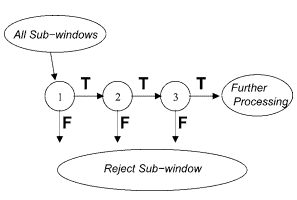
\includegraphics[width=0.6\textwidth]{gambar/cascade}
  \caption{\textit{Workflow} dari \emph{Attentional Cascade}}
\end{figure}

\emph{Attentional Cascade} adalah sebuah \emph{cascade} dari banyak 
\emph{classifier} yang dibuat untuk meningkatkan performa deteksi dengan secara radikal mengurangi jumlah 
komputasi. Intinya \emph{weak classifier} yang telah di-\emph{boost} dapat dibuat lebih 
kecil dan efisien, yang dapat menolak mayoritas \emph{sub-window} negatif dan 
mendeteksi sebagian besar dari \emph{sub-window} positif. \emph{Classifier} yang lebih 
sederhana digunakan untuk menolak mayoritas \emph{sub-window} sebelum \emph{classifier} 
yang lebih kompleks dipanggil untuk menurunkan tingkat \emph{false positives}.

Struktur dari \emph{cascade} merefleksikan 
fakta bahwa pada gambar apapun mayoritas \emph{sub-window} pasti negatif. 
Oleh karena itu, \emph{cascade} berusaha untuk sebanyaknya menolak sub-window 
negatif pada tahapan seawal mungkin. Sementara hasil positif 
akan memicu evaluasi dari setiap \emph{classifier} dalam \emph{cascade}, 
hal ini sangatlah langka.

Layaknya sebuah \emph{Decision Tree}, sebuah \emph{classifier} dilatih menggunakan 
contoh-contoh yang telah berhasil melewati tahap sebelumnya. Oleh karenanya, 
\emph{classifier} pada tahap kedua menghadapi tantangan yang jauh lebih sulit 
daripada yang pertama.

\emph{Cascade} dimulai dengan membuat sebuah \textit{stage} awal, dimana \textit{weak classifier} 
ditambahkan secara perlahan hingga \emph{detection rate} yang dituju sampai. \emph{Detection rate} 
ini harus disesuaikan oleh pengguna sesuai dengan keperluannya, tujuannya tetap untuk mengurangi 
waktu komputasi tapi juga mencoba agar tidak terlalu banyak kasus \emph{false positive} yang dapat 
lewat.

% \begin{algorithm}
%   \caption{Algoritma Pelatihan Untuk Pembuatan \textit{Cascaded Detector}}
%   \begin{algorithmic} [1]
%     \State Pengguna memilih nilai dari \textit{f}, nilai maksimum \emph{false positive} 
%     pada setiap tahap yang dapat diterima, dan \textit{d}, nilai minimum \emph{detection rate} 
%     per tahap yang dapat diterima
%     \State Pengguna memilih target keseluruhan \emph{false positive rate}, $F_{target}$
%     \State \textit{P} = kumpulan contoh positif
%     \State \textit{N} = kumpulan contoh negatif
%     \State $F_0 = 1.0; D_0 - 1.0$
%     \State $i = 0$
%     \State $while F_i > F_{target}$
%     \Statex $-i \leftarrow i + 1$
%     \Statex $-n_i = 0; F_i = F_i-_1$
%     \Statex -while $F_i > f x F_i-_1$
%     \begin{itemize}
%       \item $n_i \leftarrow n_i + 1$
%       \item Gunakan \textit{P} dan \textit{N} untuk melatih sebuah \emph{classifier}
%       dengan fitur $n_i$ menggunakan \emph{Adaboost} 
%       \item Evaluasi \emph{cascade classifier} dengan \textit{set} validasi
%       untuk menentukan $F_i$ dan $D_i$. 
%       \item kurangi \textit{threshold} untuk \emph{classifier} ke-$i$ sampai 
%       \emph{cascade classifier} memiliki tingkat deteksi paling tidak $d x D_i-_1$ 
%       (hal ini juga akan mempengaruhi $F_i$)
%     \end{itemize}
%     \Statex $-N \leftarrow$ {\O}
%     \Statex -if $F_i > F_target$ evaluasi \emph{cascade detector} menggunakan 
%     \textit{set} negatif dan masukan semua deteksi gagal ke \textit{set} N
%   \end{algorithmic}
% \end{algorithm}


%!TEX root = ./template-skripsi.tex
%-------------------------------------------------------------------------------
%                     BAB III
%               			PEMBAHASAN
%-------------------------------------------------------------------------------

\chapter{METODOLOGI PENELITIAN}

\section{Tahapan Penelitian}

Gambar \textit{flowchart} berikut mengilustrasikan proses pelatihan 
 dari dataset dan juga proses penggunaan yang sesungguhnya.

\begin{figure}[H]
  \centering{}
	\includegraphics[width=0.6\textwidth]{gambar/flowchart\_1\_1}
  \caption{Diagram alir untuk algoritma pelatihan klasifikasi objek}
\end{figure}

\begin{figure}[H]
  \centering{}
	\includegraphics[width=0.6\textwidth]{gambar/flowchart\_2}
  \caption{Diagram alir untuk algoritma pendeteksian objek}
\end{figure}

%(Jelasin disini secara ringkas, biar gak terlalu ambigu)

\section{Desain Sistem}

Dalam proses pembuatan \emph{classifier} perlu dilewati tahapan \textit{training}. 
Tujuan \textit{training} adalah untuk menciptakan suatu \emph{strong classifier} 
yang nantinya dapat digunakan untuk melakukan klasifikasi yang sebenarnya.
Pertama, gambar yang akan menjadi \textit{set} latihan dianotasi sesuai kelasnya masing-masing, 
\textit{set} latihan ini juga berisikan gambar-gambar yang tidak memiliki kelas yang benar, atau 
\emph{false example}. Setelah itu gambar melalui proses \emph{pre-processing} dan disesuaikan 
untuk mengoptimalkan proses pelatihan. Setiap gambar latihan nantinya akan 
diubah menjadi \emph{integral image} untuk dapat diproses.

Pertama algoritma akan mengkonstruksi sebuah \emph{decision tree} untuk setiap 
\emph{weaklearn} dimana \emph{branch} untuk setiap kelas akan ditentukan. Lalu 
\emph{Adaboost} akan menentukan bobot dari setiap \emph{weaklearn} dalam menentukan hasil akhir 
klasifikasi gambar. Terakhir, \emph{Adaboost} akan membuat sebuah 
\emph{strong classifier} dengan membuat sebuah \emph{Attentional Cascade}

Dengan \emph{strong classifier}, klasifikasi objek yang sesungguhnya bisa dilakukan. 
Pertama gambar yang akan dideteksi akan melalui \emph{pre-processing}. 
Kemudian \emph{integral image} akan dihitung untuk 
menghasilkan \emph{sub-window} pada gambar. setiap sub-window akan dicek menggunakan 
\emph{strong classifier}. \emph{Sub-window} yang ditemukan memiliki objek yang 
dicari akan dibuatkan \emph{bounding box} pada kelilingnya. Setelah semua 
\emph{sub-window} diperiksa, semua \emph{bounding box} yang bertindihan akan 
digabungkan sebelum gambar hasil dikembalikan ke pengguna.

\section{Training \emph{Strong Classifier}}

Pada \textit{Training} ada tiga tahapan yang perlu dijalankan 
untuk menghasilkan sebuah \emph{Strong Classifier}, 
yaitu penginputan \textit{dataset} pelatihan yang sudah dianotasi, 
pembuatan \emph{decision tree} untuk setiap fitur, 
\emph{Boosting }dan pemilihan fitur oleh Adaboost untuk membuat \emph{attentional cascade}.

\subsection{\textit{Input Dataset} Pelatihan}

\begin{figure}[H]
  \centering{}
	\includegraphics[width=0.6\textwidth]{gambar/dataset\_2}
  \caption{Contoh gambar Abudefduf, Amphiprion, Chaetodon dan contoh gambar-gambar negatif}
\end{figure}

\textit{Dataset} yang akan dipakai diambil dari fishR (Dapat dilihat di https://github.com/mekas/fishR) yang 
berisikan gambar ikan genus Abudefduf, Amphiprion dan Chaetodon. Selain itu 
\textit{dataset} juga akan ditambahkan dari hasil penelitian lapangan 
secukupnya, dengan mempertimbangkan waktu komputasi pada tahap 
pelatihan.
Untuk contoh pelatihan kelas-kelas ikan adalah gambar berukuran 72x41 piksel, 
dengan warna grayscale. Selain itu juga akan dipilih contoh 
pelatihan negatif atau kumpulan gambar yang tidak terdapat kelas 
ikan dari http://www.vision.caltech.edu/datasets/ dengan jumlah yang sama, resolusi sama dan perlakuan 
yang sama. Anotasi dilakukan dengan rumus $(x_1, y_1),...,(x_n, y_n)$ dimana 
$y_i \in Y = {1,...,k}$, $k$ disini adalah kelas-kelas yang ada dimana $y_i = 0$ 
direservasi untuk kelas negatif dan angka-angka setelahnya untuk kelas-kelas lainnya.
\textit{Dataset} ini lalu 
akan dibagi menjadi tiga yaitu \textit{training dataset}, 
\textit{validation dataset}, dan \emph{test dataset} dengan jumlah yang sama.
Nilai bobot pada tiap \textit{dataset} akan di inisialisasi dengan rumus:
\begin{equation}
  w^1_i = D(i) \text{ for } i=1,...,N
\end{equation}
dimana $w$ adalah bobot, $D$ Distribusi dan $N$ jumlah contoh pelatihan.

\subsection{Pembuatan \textit{Integral Image}}

Untuk pembuatan \emph{Integral Image}, pertama perlu dicari nilai piksel
baris pertama dan kolom pertama dari gambar. Nilai pada matriks \emph{Integral Image} 
adalah median dari nilai RGB pada piksel tersebut, namun dikarenakan warna 
gambar sudah dirubah menjadi \emph{greyscale} maka nilai pada setiap piksel 
hanya akan berupa bilangan bulat dikisaran 0 sampai 255. Nilai pada kolom 
pertama hanyalah penjumlahan nilai piksel dari piksel $(0, 0)$ sampai ke piksel 
$(0, j)$, sementara nilai pada baris pertama juga hanya penjumlahan nilai 
piksel dari $(0, 0)$ ke  $(i, 0)$. Nilai-nilai piksel lainnya lalu dapat 
dihitung menggunakan rumus: 
\begin{equation}
  \begin{split}
    \text{integral image } (i,j) = {} & \text{integral image } (i-1,j) + \text{integral image } (i,j-1) - \\
    & \text{integral image } (i-1,j-1) + \text{nilai dari piksel } (i,j)
  \end{split}
\end{equation}
Atau jumlah semua nilai piksel dari $(0, 0)$ sampai ke $(i, j)$.
Pembuatan \emph{integral image} nantinya akan digunakan oleh fitur sebagai \textit{input}.

\begin{figure}[H]
  \centering{}
	\includegraphics[width=0.6\textwidth]{gambar/integral\_image\_3}
  \caption{Gambaran \emph{integral image} dari gambar sebuah bidak catur.}
\end{figure}

\subsection{Pembuatan \textit{Features}}

Fitur-fitur yang akan digunakan dalam klasifikasi dibuat 
berdasarkan \emph{Haar-like Features} dan berisikan informasi 
lokasinya pada \emph{sub-window} dan titik-titik \emph{integral image}. 
Misalnya sebuah fitur dua persegi dengan persegi putih di 
sebelah kiri, fitur tersebut memerlukan 
nilai \emph{integral image} dari pojok kiri atas persegi putih, 
pojok kiri bawah persegi putih,  
pojok kanan atas persegi putih, 
pojok kanan bawah persegi putih, 
, pojok kanan atas persegi hitam, 
dan pojok kanan bawah persegi hitam. 
\begin{figure}[H]
  \centering{}
	\includegraphics[width=0.6\textwidth]{gambar/integral\_image\_4}
  \caption{Nilai yang diperlukan oleh fitur dua persegi, direpresentasi sebagai A, B, C, dan D}
\end{figure} 
Keenam nilai tersebut dapat digunakan untuk mencari nilai 
fitur dengan rumus:

\begin{equation}
  \begin{split}
    &\text{integral image E} - \text{integral image B} - \text{integral image D} + \text{integral image A} \\
    & - \text{integral image F} - \text{integral image C} - \text{integral image E} + \text{integral image B} \\    
  \end{split}
\end{equation}

Pada tahap ini \emph{integral image} yang dipilih akan dibuat untuk semua 
posibilitas lokasi yang ada dan ukuran yang ada. Hal ini dilakukan dengan 
membuat fitur dimulai dari kiri atas gambar dengan ukuran 20 x 20 piksel untuk fitur 
dua persegi, dan 20 x 30 piksel untuk fitur tiga persegi, sampai pojok kanan bawah. 
Hal ini juga dilakukan untuk ukuran-ukuran yang lebih besar sampai fitur lebih besar 
dari \emph{sub-window} yang digunakan dan tidak bisa muat lagi didalan \emph{sub-window}. 
Ukuran paling kecil dari fitur akan disesuaikan pada saat penelitian 
bila ternyata fitur terlalu banyak dan memperlambat proses pelatihan. 

\subsection{Pembuatan \textit{Decision Tree}}

Setiap \emph{weaklearner} adalah sebuah \emph{decision tree} yang mengambil nilai 
dari \emph{Haar-like features} sebagai variabel klasifikasi.
\emph{Haar-like features} dapat mengembalikan 
sebuah nilai perbandingan intensitas cahaya dari suatu area pada gambar dan 
mendeteksi keberadaan suatu \emph{fitur} seperti 
perbedaan warna, garis, maupun perbedaan kontras pada gambar. 
%(Jelasin step by step pembuatan decision tree pake algoritma).

\subsection{\emph{Boosting}}

Algoritma \emph{Adaboost} akan mem-\emph{boosting} \emph{weaklearner} untuk 
menciptakan sebuah \emph{strong classifier}. \emph{Boosting} dilakukan dari 
\emph{weaklearner} yang memiliki tingkat akurasi paling tinggi, dan dengan 
menggunakan \emph{dataset} latihan.

\emph{Adaboost} akan menjalankan \emph{weaklearner} terbaik untuk 
mengklasifikasi seluruh contoh \emph{dataset} latihan dan mencatat contoh yang 
gagal diklasifikasi oleh \emph{weaklearner} tersebut. 
Nilai dari \emph{weaklearner} 
tersebut dihitung dengan:
\begin{equation}
  sum(N)(i=1) w^t_i.1(h(x_i)\ne y_i)
\end{equation} 
dimana $N$ adalah jumlah total contoh latihan, $D_t$ adalah distribusi bobot pada 
iterasi $t$, $w^t_i$ adalah nilai bobot contoh ke-$i$ pada iterasi $t$, 
$y_i$ adalah label yang benar untuk contoh latihan ke-$i$, dan $h(x_i)$ 
adalah hasil dari \emph{weaklearn}. 
Hasilnya juga akan dicatat untuk urutan \emph{Boosting} ronde berikutnya dan 
juga sebagai nilai voting pada klasifikasi yang sebenarnya. 
Nantinya bobot dari seluruh \emph{dataset} latihan akan dihitung ulang dengan menaikan bobot dari contoh 
yang gagal diklasifikasi oleh \emph{weaklearner} sebelumnya. Proses ini dilakukan 
untuk setiap \emph{weaklearner}. 
%(Masukin rumus re-distribusi bobot contoh disini)

Ketika sebuah ronde \emph{Boosting} sudah selesai dan seluruh \emph{weaklearner} sudah  diurutkan sesuai dengan 
nilai yang didapat dari ronde tersebut. \emph{Adaboost} akan melakukan validasi 
tingkat akurasi \emph{strong classifier} yang sudah dibuat menggunakan \emph{dataset} validasi. 
hal ini dilakukan dengan membandingkan tingkat presisi \emph{strong classifer} 
yang dihasilkan ronde ini dengan \emph{strong classifer} yang dihasilkan ronde 
sebelumnya. Bisa tingkat presisi ternyata semakin berkurang, maka \emph{Boosting} 
akan dihentikan dan \emph{strong classifier} 
%(ronde ini atau sebelumnya, cek lagi) 
menjadi \emph{final strong classifier}.

\subsection{Pembuatan \emph{Attentional Cascade}}

\begin{figure}[H]
  \centering{}
	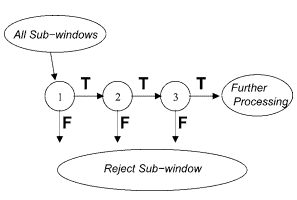
\includegraphics[width=0.6\textwidth]{gambar/cascade}
  \caption{\textit{Workflow} dari \emph{Attentional Cascade}}
\end{figure}

Sebelum pembuatan \emph{attentional cascade}, \emph{weaklearner} yang kurang 
diskriminatif akan dibuang. 
%Hal ini dilakukan dengan (cari, karena bagian ini 
%belum jelas dari kemarin). 
\emph{Attentional cascade} akan dibuat dari \emph{weaklearner} 
yang tersisa secara bertahap. 
Pertama, target \textit{false positive} pada setiap \emph{cascade} 
harus ditentukan oleh pengguna. \emph{Framework VIola-Jones} menggunakan target 
\textit{false positive} 50\% untuk \emph{cascade} pertama, dan 
\textit{false positive} 80\% untuk semua \emph{cascade} setelahnya.
Target \textit{false posiive} ini akan disesuaikan 
saat penelitian lapangan, bila target akurasi tidak berhasil dicapai 
dengan target \textit{false positive} sebelumnya.
Pada setiap fase \emph{cascade}, \emph{weaklearner} akan 
ditambahkan satu-persatu. Setiap sebuah \emph{weaklearner} ditambahkan, tes akan dilakukan 
dengan \emph{dataset} tes. \emph{Weaklearner} akan terus ditambahkan hingga \emph{false positive rate} 
yang ditentukan untuk fase itu dicapai. Fase akan terus bertambah hingga 
akurasi sempurna dicapai, atau hingga \emph{weaklearner} sudah habis. 
%(Ini periu dijabarin lagi dengan rumus per-step). 


\section{Skenario Eksperimen dan Validasi}

Tahapan ini adalah penggunakaan \emph{classifier} yang sebenarnya dengan tujuan 
memvalidasi akurasi dari \emph{classifier} tersebut. 
Gambar ikan yang akan dipakai dalam proses validasi akan 
melalui beberapa langkah dalam tahap ini, 
yaitu: \textit{Pre-processing} dalam bentuk \emph{grayscaling}, Penghitungan 
\emph{Integral Image}, dan deteksi yang sesungguhnya menggunakan \emph{strong classsifier} 
yang telah dibuat dengan metode Sliding Window.

\subsection{\textit{Pre-processing} dan Penghitungan \emph{Integral Image}}

Untuk klasifikasi sebenarnya, gambar \emph{input} akan diproses terlebih dahulu. 
Gambar awalnya akan melakui proses \textit{pre-processing} dan dirubah kedalam warna 
\emph{grayscale} %(Jelasin perubahan greyscale ini kayak gimana) 
untuk mempermudah penghitungan dengan bantuan \emph{library OpenCV}. 
Setelah tu sebuah matriks sebesar resolusi gambar akan dibuat untuk 
penghitungan \emph{Integral Image} yang nantinya akan mempercepat proses 
penghitungan fitur. Pembuatan \emph{integral image} pada tahap ini sama persis 
dengan pembuatan pada tahap pelatihan.

\subsection{Klasifikasi}

Pada tahap ini, gambar yang sudah berubah dalam bentuk 
\emph{integral image} akan diklasifikasi menggunakan 
\emph{strong classifier}. \emph{Strong classifier} akan berjalan dari 
pojok kiri atas gambar, atau piksel pertama, mencoba untuk mengklasifikasi 
sebuah \emph{sub-window} berukuran 72x41 piksel. Bila posisi tersebut sudah 
selesai diklasifikasi, terlepas hasilnya, \emph{sub-window} akan 
bergerak ke kanan sebanyak satu piksel dan mengklasifikasi area baru tersebut. 
Hal ini akan terus berlanjut hingga \emph{sub-window} bisa dibuat lagi ke kanan. 
Bilama demikian \emph{sub-window} akan kembali ke ka kanan, namun kali ini 
diturunkan sebanyak satu piksel. Pergerakan \emph{sliding window} ini 
bertujuan agar seluruh bagian dari gambar dapat terklasifikasi.

\begin{figure}[H]
  \centering{}
	\includegraphics[width=0.6\textwidth]{gambar/sliding\_window\_1}
  \caption{Gambaran ukuran \emph{sub-window} 72x41 piksel pada gambar 300x220}
\end{figure}

Jika \emph{sub-window} dengan ukuran 72x42 piksel sudah mengklasifikasi 
seluruh bagian gambar hingga pojok kanan bawah, maka \emph{sub-window} 
akan diperbesar dengan faktor 1.25 dan proses dimulai lagi dari pojok kiri atas. 
Selain itu ukuran dan lokasi dari \emph{feature} akan disesuaikan untuk mangakomodasi 
\emph{sub-window} yang sudah diperbesar. Hal ini dilakukan untuk mengklasifikasi 
objek yang memiliki ukuran berbeda didalam gambar.

\subsection{Anotasi}

\begin{figure}[H]
  \centering{}
	\includegraphics[width=0.6\textwidth]{gambar/sliding\_window\_2}
  \caption{Gambaran \textit{sub-window} yang berhasil mengklasifikasi ikan didalam gambar}
\end{figure}

Setelah semua \textit{sub-window} sudah diklasifikasi dengan menggunakan 
\emph{strong classifier}. Algoritma akan menggambarkan di lokasi \textit{sub-window} 
yang positif terklasifikasi (Memiliki salah satu kelas ikan yang telah dilatih ke \emph{strong classifier}), 
\emph{bounding box} untuk menganotasi kelasnya. Pengguna lalu dapat menentukan 
dari hasil anotasi bilamana target akurasi sudah tercapai.



% %!TEX root = ./template-skripsi.tex
%-------------------------------------------------------------------------------
%                            	BAB IV
%               		KESIMPULAN DAN SARAN
%-------------------------------------------------------------------------------

\chapter{HASIL DAN PEMBAHASAN}

\section{\textit{Training Strong Classifier}}
\subsection{\textit{Input} Gambar dan \textit{labeling}}

	\begin{figure}[H]
		\centering{}
		\includegraphics[width=0.6\textwidth]{gambar/training\_data}
		\caption{Gambar-gambar yang akan dipakai untuk training}
	\end{figure}

	Langkah pertama dalam melatih \textit{classifier} adalah dengan memasukan 
	\textit{dataset} untuk latihan berserta label-labelnya. Gambar pertama dimasukan 
	ke dalam folder sesuai dengan kelasnya. Dalam situasi ini ada empat folder yaitu, 
	untuk kelas satu: abudefduf, untuk kelas dua: amphiprion, untuk kelas tiga: chaetodon 
	dan terakhir untuk kelas nol: negative\_examples. Gambar-gambar tersebut lalu akan dibaca 
	menggunakan \textit{library} CV2 yang bertugas juga untuk mengubah gambar menjadi 
	\textit{greyscale}. Berikut adalah \emph{source code} \texttt{load\_images()}
	yang digunakan untuk membaca set gambar latihan:

	\begin{figure}[H]
		\begin{lstlisting}[language=Python, basicstyle=\tiny]
			def load_images(directory):
				images=[]
				labels=[]
				for filename in os.listdir(directory):
					if filename.endswith(".png"):
						image_path = os.path.join(directory, filename)
						image = cv2.imread(image_path, cv2.IMREAD_GRAYSCALE)
						image = cv2.resize(image, (350, 200))
						images.append(image)
						labels.append(get_label(directory))
				return np.array(images), np.array(labels)
		\end{lstlisting}
		\caption{\emph{source code:} \textit{read} gambar, labelisasi, pengubahan ke \textit{greyscale}, 
		dan memastikan ukuran gambar 350 x 200 piksel}
		\label{code:pre-processing gambar}
	\end{figure}

	\begin{figure}[H]
		\begin{lstlisting}[language=Python, basicstyle=\tiny]
			def get_label(directory):
				# add more to add more class
				if directory == "fish_dataset\\abudefduf": return 1
				if directory == "fish_dataset\\amphiprion": return 2
				if directory == "fish_dataset\\chaetodon": return 3
				else: return 0
		\end{lstlisting}
		\caption{\emph{source code:} labelisasi gambar sesuai dengan foldernya}
		\label{code:labeling}
	\end{figure}

	Untuk memanggil kedua fungsi \texttt{load\_images} dan \texttt{get\_label} diperlukan sebuah fungsi lainnya 
	yang berfungsi juga untuk menggabungkan semua gambar dan label menjadi dua buah \emph{array} 
	\texttt{images} dan \texttt{labels}. Kedua \emph{array} ini nantinya akan menjadi \textit{dataset} utama 
	dalam proses pelatihan. Berikut \emph{source code} dari \texttt{combine\_dataset} yang 
	digunakan untuk membuat \textit{array} \texttt{images} dan \texttt{labels}:

	\begin{figure}[H]
		\begin{lstlisting}[language=Python, basicstyle=\tiny]
			def combine_dataset():
				# load datasets from directories
				# add class to get_label first or the class will be considered a negative example
				abudefduf_images, abudefduf_labels = load_images("fish_dataset\\abudefduf")
				amphiprion_images, amphiprion_labels = load_images("fish_dataset\\amphiprion")
				chaetodon_images, chaetodon_labels = load_images("fish_dataset\\chaetodon")
				negatives_images, negatives_labels = load_images("fish_dataset\\negative_examples")

				# combining into a single dataset
				images = np.concatenate((abudefduf_images, amphiprion_images, chaetodon_images, negatives_images), axis = 0)
				labels = np.concatenate((abudefduf_labels, amphiprion_labels, chaetodon_labels, negatives_labels), axis = 0)

				return images, labels
		\end{lstlisting}
		\caption{\emph{source code:} \textit{load} gambar-gambar dari folder yang bersangkutan dan 
		menggabungkannya}
		\label{code:conc dataset}
	\end{figure}

\subsection{\textit{Generate Haar-like Features}}
	Untuk melakukan \emph{generate feature} sebuah fungsi bernama \texttt{generate\_features()} dipanggil 
	dengan parameter lebar dan tinggi dari \emph{sub-window} yang akan digunakan. Fungsi ini akan 
	menghasilkan kurang lebih sekitar 520000 fitur berbeda untuk \emph{sub-window} berukuran 
	50 x 50 piksel. Berikut \emph{source code}-nya:

	\begin{figure}[H]
		\begin{lstlisting}[language=Python, basicstyle=\tiny]
			def generate_features(image_height, image_width):
				features = []
				features_list = ["Two Horizontal", "Two Vertical", "Four Diagonal", "Right Triangular", "Left Triangular", "Three Horizontal", "Three Vertical"]
				for i in features_list:
					match i:
						case "Two Horizontal" | "Two Vertical" | "Four Diagonal" | "Right Triangular" | "Left Triangular":
							feature_height = 4
							feature_width = 4
						case "Three Horizontal":
							feature_height = 4
							feature_width = 6
						case "Three Vertical":
							feature_height = 6
							feature_width = 4
					for w in range (feature_width, image_width+1, feature_width):
						for h in range (feature_height, image_height+1, feature_height):
							for x in range (0, image_width - w):
								for y in range (0, image_height - h):
									feature = (i, x, y, w, h)
									features.append(feature)
    			return features
		\end{lstlisting}
		\caption{\emph{source code:} sebuah data dalam \textit{features} memiliki semua informasi yang diperlukan 
		untuk melakukan perhitungan nilai sebuah fitur. Tipe-tipe fitur akan menentukan rumus perhitungan fitur tersebut}
		\label{code:generate features}
	\end{figure}

\subsection{\textit{Calculating all features of all images}}
	Untuk mempermudah proses pembuatan \emph{Decision tree} nantinya, semua fitur 
	pada semua \textit{sub-window}, pada semua gambar akan dihitung dan dimasukan 
	kedalam sebuah dokumen .CSV mengunakan \textit{library} Pandas. Fungsi yang dipakai untuk memulai proses ini adalah 
	fungsi \texttt{write\_csv()} pada Utilities.py. Berikut \emph{source code}-nya:

	\begin{figure}[H]
		\begin{lstlisting}[language=Python, basicstyle=\tiny]
			def write_csv(images, labels, features, csv_name):
				print("starting write_csv")
				for window_num in range(3):
					temp_window_values = np.zeros((len(images), len(features)), dtype=object)
					image_ids = np.arange(len(images))

					for i in range(len(images)):
						new_data = Dataset(images[i], labels[i], features)
						if window_num == 0:
							temp_window_values[i] = new_data.window_1_features
						elif window_num == 1:
							temp_window_values[i] = new_data.window_2_features
						elif window_num == 2:
							temp_window_values[i] = new_data.window_3_features

					window_feature = {'image_ids': image_ids}
					for i in range(len(features)):
						column_name = f'win_{window_num + 1}_feature_{i}'
						window_feature[column_name] = temp_window_values[:, i]

					directory = f"Data/{csv_name}_window_{window_num}.csv"

					window_feature = pd.DataFrame(window_feature)
					window_feature.to_csv(directory, index=False)
				print("csv write complete!")
		\end{lstlisting}
		\caption{\emph{source code:} \texttt{write\_csv()} mengambil semua gambar, 
		label, fitur dan mengkalkulasi semua fitur untuk ketiga \textit{sub-window}}
		\label{code:calculate all features}
	\end{figure}

	Fungsi ini menghasilkan sebuah dokumen .csv untuk setiap \textit{sub-window} dengan
	baris mengikuti jumlah gambar didalam \textit{dataset} dan kolom mengikuti jumlah fitur yang ada. 
	Maka dari itu untuk \emph{dataset} 80 gambar akan dihasilkan sebuah tabel .csv dengan 
	bentuk 80 x 520.000.

	Fungsi ini berjalan cukup lama dengan jumlah gambar 80 buah. Penulis menghitung rata-rata 
	waktu yang diperlukan bagi fungsi untuk membuat sebuah dokumen .csv adalah 45 menit minimum. 
	Dan proses ini dilakukan sampai tiga kali agar dapat menciptakan tiga dokumen .csv untuk ketiga 
	\textit{sub-window}. Dokumen .csv ini nantinya akan diperlukan untuk proses pembuatan \emph{decision tree}.

	\texttt{Dataset} adalah sebuah \textit{class} yang digunakan untuk menyimpan seluruh nilai fitur 
	dari sebuah gambar sebelum dimasukan kedalam dokumen .csv .  
	Berikut adalah bentuk \textit{class} \texttt{Dataset} berserta 
	fungsi bawaannya \texttt{Find\_Feature\_Value}:

	\begin{figure}[H]
		\begin{lstlisting}[language=Python, basicstyle=\tiny]
			class Dataset:
				def __init__(self, image, label, feature_list):
					self.image = image
					self.label = label
					self.window_1_features = self.Find_Feature_Value(image, feature_list, self.class_Window_offset_1[label][0], self.class_Window_offset_1[label][1])
					self.window_2_features = self.Find_Feature_Value(image, feature_list, self.class_Window_offset_2[label][0], self.class_Window_offset_2[label][1])
					self.window_3_features = self.Find_Feature_Value(image, feature_list, self.class_Window_offset_3[label][0], self.class_Window_offset_3[label][1])

				def Find_Feature_Value(self, image, feature_list, x_offset, y_offset):
					features = np.zeros(len(feature_list), dtype=object)
					for i in range(len(feature_list)):
						feature_type, x, y, width, height = feature_list[i]
						x += x_offset
						y += y_offset
						updated_feature = (feature_type, x, y, width, height)
						data_features = compute_feature_with_matrix(image, 0, updated_feature)
						features[i] = data_features
					return features
				
		\end{lstlisting}
		\caption{\emph{source code:} \textit{class Dataset}}
		\label{code:Dataset class}
	\end{figure}

	\texttt{Dataset}, untuk melakukan perhitungan fitur, digunakan \textit{Offset} 
	menspesifikasi lokasi mulut, sirip dan ekor ikan pada gambar. Hal ini dilakukan 
	karena masing-masing kelas ikan semuanya memiliki 
	mulut, sirip dan ekor dengan lokasi yang berbeda satu dengan yang lainnya. Contohnya: Mulut dari spesies ikan Chaetodon 
	agak lebih kebawah dibandingkan kedua kelas ikan lainnya. Selain itu juga untuk setiap bagian 
	ikan yang akan diklasifikasi akan dicari lokasi yang paling terlihat unik daripada kelas-kelas lainnya. Contohnya 
	pada kelas spesies ikan Abudefduf diambil bagian ekor yang memberntuk huruf "V" 
	sementara pada kelas spesies Amphiprion bagian kelas yang dipelajari adalah 
	bagian melengkung bagian atas diantara ekor dan badan. Berikut adalah 
	\textit{offset} yang penulis gunakan untuk pelatihan:

	\begin{figure}[H]
		\begin{lstlisting}[language=Python, basicstyle=\tiny]
			class_Window_offset_1 = [
				# order according to label's order in LoadImages
				# for searching mouth features
				(0, 0),
				(0, 88),
				(0, 73),
				(15, 100)
			]

			class_Window_offset_2 = [
				# order according to label's order in LoadImages
				# for searching fin features
				(0, 0),
				(116, 0),
				(153, 9),
				(116, 0)
    
			]

			class_Window_offset_3 = [
				# order according to label's order in LoadImages
				# for searching tail feature
				(0, 0),
				(280, 89),
				(237, 47),
				(277, 80)
    ]
		\end{lstlisting}
		\caption{\emph{source code:} \textit{offset} ini di-inisalisasi untuk setiap kelas Dataset 
		sehingga bisa diakses langsung oleh fungsi \texttt{Find\_Feature\_Value}}
		\label{code:Training sub-window offset}
	\end{figure}

	Untuk perhitungan nilai fitur dari gambar digunakan fungsi \texttt{compute\_feature\_with\_matrix()}. 
	Pertama data fitur diubah dengan menambah lokasi x dan y dari fitur dengan \texttt{x\_offset}, dan  \texttt{y\_offset} 
	lalu fitur akan mengembalikan sebuah nilai float dari hasil perhitungan tersebut. Berikut \emph{source code} 
	dari \texttt{compute\_feature\_with\_matrix}:
	
	\begin{figure}[H]
		\begin{lstlisting}[language=Python, basicstyle=\tiny]
			def compute_feature_with_matrix(image, feature):
				feature_type, x, y, width, height = feature
				# +1 due to slicing paramter = start at:stop before
				match feature_type:
					case "Two Horizontal":
						white = np.sum(image[y:y + height + 1, x:x + int(width/2) + 1])
						black = np.sum(image[y:y + height + 1, x + int(width/2):x + width + 1])
					case "Two Vertical":
						white = np.sum(image[y:y + int(height/2) + 1, x:x + width+1])
						black = np.sum(image[y + int(height/2):y + height + 1, x:x + width+1])
					case "Three Horizontal":
						white = np.sum(image[y: y + height + 1, x:x + int(width/3) + 1]) + np.sum(image[y: y + height + 1, x + int(width*2/3):x + width + 1])
						black = np.sum(image[y: y + height + 1, x + int(width/3):x + int(width*2/3) + 1])
					case "Three Vertical":
						white = np.sum(image[y:y + int(height/3) + 1, x:x + width + 1]) + np.sum(image[y + int(height*2/3):y + height + 1, x: x + width + 1])
						black = np.sum(image[y + int(height/3):y + int(height*2/3) + 1, x:x + width + 1])
					case "Four Diagonal":
						white = np.sum(image[y:y + int(height/2) + 1, x + int(width/2): x + width + 1]) + np.sum(image[y + int(height/2):y + height + 1, x: x + int(width/2) + 1])
						black = np.sum(image[y:y + int(height/2) + 1, x:x + int(width/2) + 1]) + np.sum(image[y + int(height/2): y + height + 1, x + int(width/2):x + width + 1])
					case "Right Triangular":
						matrix = image[y:y + height + 1, x:x + width + 1]
						white = np.sum(np.tril(matrix))
						black = np.sum(np.triu(matrix))
					case "Left Triangular":
						matrix = np.rot90(image[y:y + height + 1, x:x + width + 1], k=3)
						white = np.sum(np.tril(matrix))
						black = np.sum(np.triu(matrix))
				return int(white) - int(black)
		\end{lstlisting}
		\caption{\emph{source code:} \textit{offset} ini di-inisalisasi untuk setiap kelas Dataset 
		sehingga bisa diakses langsung oleh fungsi \texttt{Find\_Feature\_Value()}}
		\label{code: feature calculation}
	\end{figure}

	\subsection{\textit{Create Decision Tree for each Feature}}
		Setelah semua nilai fitur sudah dihitung dan dimasukan kedalam dokumen .csv, 
		selanjutnya bisa dimulai proses pembuatan \emph{decision tree} atau \emph{weak classifier}. 
		Proses ini dimulai dengan pertama membagi contoh menjadi tiga kelompok, yaitu data \emph{training}, 
		data \emph{testing} dan data \emph{validation}. Hal ini dilakukan dengan menggunakan fungsi 
		\texttt{split\_data} dibantu dengan fungsi \texttt{train\_test\_split()} dari \textit{library} sklearn:

		\begin{figure}[H]
			\begin{lstlisting}[language=Python, basicstyle=\tiny]
				def split_data(features, csv_name, labels):
					data = DecisionTree.get_data(features, csv_name)
					labels_df = pd.DataFrame({'Label' : labels})
					data = pd.concat([data, labels_df], axis=1)

					X = data.iloc[:, :-1].values 
					Y = data.iloc[:, -1].values.reshape(-1, 1)

					X_temp, X_train, Y_temp, Y_train = train_test_split(X, Y, test_size=0.3, random_state=42)
					X_valid, X_test, Y_valid, Y_test = train_test_split(X_temp, Y_temp, test_size=0.5, random_state=42)

					print(type(X_train))
					splits = [X_train, Y_train, X_test, Y_test, X_valid, Y_valid]
					return splits
			\end{lstlisting}
			\caption{\emph{source code:} data \emph{training}, data \emph{testing} dan data \emph{validation} 
			disimpan kedalam \textit{array} \texttt{X\_train, Y\_train, X\_test, Y\_test, X\_valid, Y\_valid}. 
			Yang lalu disimpan kedalam \texttt{splits}}
			\label{code: spliting dataset}
		\end{figure}

		Label baru ditambahkan sekarang agar tidak menggangu proses penulisan kolom .csv yang dinamis 
		mengikuti jumlah fitur yang ada. Hasilnya adalah sebuah \textit{object} bernama \texttt{splits} 
		yang memiliki \textit{dataframe}: \texttt{X\_train, Y\_train, X\_test, Y\_test, X\_valid, Y\_valid}. \textit{Dataframe} 
		dengan data awalan X berisikan nilai-nilai fitur yang sudah dikalkulasi di tahap sebelumnya. 
		Sementara data awalan Y berisikan label untuk data X.

		\texttt{split\_data()} mengambil data dari .csv menggunakan fungsi bernama \texttt{get\_data}. Fungsi ini 
		hanya bertugas untuk membaca .csv saja dengan bantuan fungsi \texttt{read\_csv} dari \textit{library} Pandas:
		
		\begin{figure}[H]
			\begin{lstlisting}[language=Python, basicstyle=\tiny]
				def get_data(features, csv_name):
					col_names = ['image_ids']
					for i in range(len(features)):
						temp_column_name = f'win_1_feature_{i}'
						col_names.append(temp_column_name)
					return Utilities.read_csv(csv_name, col_names)

				def read_csv(csv_name, col_names):
					# used to read all column
					directory = "Data/" + csv_name + ".csv"
					data = pd.read_csv(directory, skiprows=1, header=None, names = col_names)
					return data
			\end{lstlisting}
			\caption{\emph{source code:} get data dan readcsv yang digunakan oleh split data}
			\label{code: get data and read csv}
		\end{figure}

		setelah data di-\textit{split}, barulah \emph{decision tree} bisa deibuat dengan menggunakan 
		fungsi \texttt{build\_all\_tree}:

		\begin{figure}[H]
			\begin{lstlisting}[language=Python, basicstyle=\tiny]
				def build_all_tree(splits, features):
					classifiers = [None] * len(features)
					classifiers_accuracy = [0] * len(features)
					X_train, Y_train, X_test, Y_test, X_valid, Y_valid = splits
					minimum_splits = 3
					maximum_depth = 3
					for i in range(len(features)):
						if i % 1000 == 0: print (f'starting tree {i}')
						classifier = DecisionTreeClassifier(minimum_splits, maximum_depth)
						classifier.fit(temp_X_train, Y_train)
						# classifier.print_tree()

						classifiers[i] = classifier
						Y_pred = classifier.predict(X_test)
						classifiers_accuracy[i] = accuracy_score(Y_test, Y_pred)
					return classifiers, classifiers_accuracy
			\end{lstlisting}
			\caption{\emph{source code:} \texttt{build\_all\_tree} untuk membuat semua decision tree untuk setiap fitur}
			\label{code: make all decision tree}
		\end{figure}

		Pada tahap ini \texttt{build\_all\_tree} mengisolasi kolom nilai fitur yang berhubungan 
		dan menyimpannya pada \texttt{temp\_X\_train}, yang nantinya akan digunakan saat pembuatan 
		\emph{decision tree}. \emph{Decision tree} di-inisialisais membuat \textit{class}
		\texttt{DecisionTreeClassifier} dan disimpan menjadi \texttt{classifier}. 
		\texttt{Classifier} lalu dilatih menggunakan fungsi \texttt{fit()}. Hasil dari pelatihan ini lalu langsung dites menggunakan 
		fungsi \texttt{accuracy\_score()} dari \textit{library} Sklearn. Variabel \texttt{classifiers\_accuracy} ini nantinya 
		akan dipakai dalam proses \emph{Boosting}. Untuk keseluruhan \textit{class} \texttt{DecisionTreeClassifier} 
		dan fungsi-fungsinya bisa dilihat berkut ini:

		\begin{figure}[H]
			\begin{lstlisting}[language=Python, basicstyle=\tiny]
				class Node():
					def __init__(self, feature_index=None, threshold=None, left=None, right=None, info_gain=None, value=None):
						self.feature_index = feature_index
						self.threshold = threshold
						self.left = left
						self.right = right
						self.info_gain = info_gain

						self.value = value
			\end{lstlisting}
			\caption{\emph{source code: class} \texttt{node} digunakan untuk menyimpan informasi cabang dan
			\textit{threshold} pada \emph{node decision tree}}
			\label{code: node class}
		\end{figure}	

		\begin{figure}[H]
			\begin{lstlisting}[language=Python, basicstyle=\tiny]

				class DecisionTreeClassifier():
					def __init__(self, minimum_splits = 2, maximum_depth = 2):
						self.root = None

						# stopping condition
						self.minimum_splits = minimum_splits
						self.maximum_depth = maximum_depth

			\end{lstlisting}
			\caption{\emph{source code: class} digunakan untuk menyimpan tinggi maksimal dan minimal 
			\textit{split} pada \emph{decision tree}. Semua data lainnya disimpan pada \texttt{node}}
			\label{code: DecisionTreeClassifier class}
		\end{figure}

		\begin{figure}[H]
			\begin{lstlisting}[language=Python, basicstyle=\tiny]
						
				def build_tree(self, training_dataset, current_depth = 0):

					X, Y = training_dataset[:,:-1], training_dataset[:,-1]
					num_samples, num_features = np.shape(X)
			
					# split until conditons are met
					if num_samples >= self.minimum_splits and current_depth <= self.maximum_depth:
						# find best split
						best_split = self.get_best_split(training_dataset, num_features)
						# check if information gain is positive
						if best_split["info_gain"]>0:
							left_subtree = self.build_tree(best_split["dataset_left"], current_depth+1)
							right_subtree = self.build_tree(best_split["dataset_right"], current_depth+1)
							return Node(best_split["feature_index"], best_split["threshold"], left_subtree, right_subtree, best_split["info_gain"])
						
					leaf_value = self.calculate_leaf_value(Y)
					return Node(value=leaf_value)
					
			\end{lstlisting}
			\caption{\emph{source code:} fungsi utama dari \emph{class} DecisionTreeClassifier}
			\label{code: build tree function}
		\end{figure}

		Fungsi \texttt{build\_tree()} adalah fungsi utama untuk pelatihan \emph{decision tree} yang berjalan secara 
		rekursif sampai sebuah daun sudah didapat, atau kedalaman maksimum sudah dicapai. 
		Sebuah daun sudah didapat bilamana \texttt{info gain} dari fungsi \texttt{get\_best\_split} adalah 0, 
		atau \textit{node} sudah tidak perlu dipecah lagi karena mencapai potensi maksimum \textit{decision tree}.

		\begin{figure}[H]
			\begin{lstlisting}[language=Python, basicstyle=\tiny]

				def get_best_split(self, dataset, num_features):
					# dictionary to save data
					best_split = {
					"info_gain": -float("inf")  # Initialize info_gain to a very small value
					} 
					max_info_gain = -float("inf")

					for feature_index in range(num_features):
						feature_values = dataset[:, feature_index]
						potential_thresholds = np.unique(feature_values)

						for threshold in potential_thresholds:
							# get curent split
							dataset_left, dataset_right = self.split(dataset, feature_index, threshold)
							# check if child not null
							if len(dataset_left) > 0 and len(dataset_right) > 0:
								y, left_y, rigth_y = dataset[:,-1], dataset_left[:,-1], dataset_right[:, -1]
								# compute information gain
								current_info_gain = self.information_gain(y, left_y, rigth_y, "gini")
								# update best split if needed
								if current_info_gain > max_info_gain:
									best_split["feature_index"] = feature_index
									best_split["threshold"] = threshold
									best_split["dataset_left"] = dataset_left
									best_split["dataset_right"] = dataset_right
									best_split["info_gain"] = current_info_gain
									max_info_gain = current_info_gain

        			return best_split

			\end{lstlisting}
			\caption{\emph{source code:} fungsi get\_best\_split}
			\label{code: get split function}
		\end{figure}

		Fungsi \texttt{get\_best\_split()} bertugas untuk mencari \textit{threshold} paling sesuai 
		untuk memecah cabang suatu \textit{node} dengan mengetes satu-persatu nilai 
		atribut dari data latihan. Atribut disini adalah nilai \textit{feature} yang sedang dilatih 
		dari semua gambar dari set \textit{train}. Untuk mencari \textit{info gain}, \textit{gini} 
		akan dihitung menggunakan fungsi \texttt{information\_gain}. Selain \textit{gini}, 
		menghitung \texttt{information gain} juga dapat dilakukan dengan menggunakan \textit{entropy}.

		\begin{figure}[H]
			\begin{lstlisting}[language=Python, basicstyle=\tiny]

					def split(self, dataset, feature_index, threshold):
						# fuction to split data 
						dataset_left = np.array([row for row in dataset if row[feature_index] <= threshold])
						dataset_rigth = np.array([row for row in dataset if row[feature_index] > threshold])
						return dataset_left, dataset_rigth
			
			\end{lstlisting}
			\caption{\emph{source code:} fungsi split hanya bertugas membagi \texttt{node} 
			berdasarkan \textit{threshold} yang sudah ditemukan}
			\label{code: split function}
		\end{figure}

		\begin{figure}[H]
			\begin{lstlisting}[language=Python, basicstyle=\tiny]
					
					def information_gain(self, parent, left_child, right_child, mode="entropy"):
						weight_left = len(left_child) / len(parent)
						weight_rigth = len(right_child) / len(parent)
						if mode == "gini":
							gain = self.gini_index(parent) - (weight_left * self.gini_index(left_child) + weight_rigth * self.gini_index(right_child))
						else:
							gain = self.entropy(parent) - (weight_left * self.entropy(left_child) + weight_rigth * self.entropy(right_child))
						return gain
					
			\end{lstlisting}
			\caption{\emph{source code:} \texttt{information\_gain()} mencari data dengan menghitung \emph{gini} 
			atau \textit{entropy}}
			\label{code: split function}
		\end{figure}
		
		\begin{figure}[H]
			\begin{lstlisting}[language=Python, basicstyle=\tiny]

					def entropy(self, y):
						# fuction to count entropy
						class_labels = np.unique(y)
						entropy = 0
						for cls in class_labels:
							p_cls = len(y[y == cls]) / len(y)
							entropy += -p_cls * np.log2(p_cls)
						return entropy
					
			\end{lstlisting}
			\caption{\emph{source code:} perhitungan \emph{entrophy}}
			\label{code: entrophy calculation function}
		\end{figure}

		\begin{figure}[H]
			\begin{lstlisting}[language=Python, basicstyle=\tiny]

					def gini_index(self, y):
						# function to count gini index (lebih cepet aja karna gak pake log)
						class_labels = np.unique(y)
						gini = 0
						for cls in class_labels:
							p_cls = len(y[y == cls]) / len(y)
							gini += p_cls**2
						return 1 - gini

			\end{lstlisting}
			\caption{\emph{source code:} perhitungan \emph{gini}}
			\label{code: gini calculation function}
		\end{figure}

		\begin{figure}[H]
			\begin{lstlisting}[language=Python, basicstyle=\tiny]

					def calculate_leaf_value(self, Y):

						Y = list(Y)
						return max(Y, key = Y.count)

			\end{lstlisting}
			\caption{\emph{source code:} fungsi untuk mencari mayoritas 
			kelas pada \textit{leaf node}}
			\label{code: find majority class in node function}
		\end{figure} 

		\begin{figure}[H]
			\begin{lstlisting}[language=Python, basicstyle=\tiny]

					def fit(self, X, Y):
						# fuction to train tree 
						dataset = np.concatenate((X, Y), axis = 1)
						self.root = self.build_tree(dataset)

			\end{lstlisting}
			\caption{\emph{source code:} fungsi \texttt{fit()} adalah fungsi 
			yang dipanggil untuk mulai membangun \emph{decision tree} setelah dibuat}
			\label{code: fit function}
		\end{figure}

		Terakhir, fungsi \texttt{Predict()} akan digunakan untuk klasifikasi yang sebenarnya. Dalam fugnsi ini 
		fit mengambil X atau \textit{dataset} \texttt{X\_test} untuk mengetes akurasi dari \emph{decision tree} 
		tersebut yang lalu akan dikomparasi dengan \texttt{Y\_test} menggunakan fungsi sklearn \texttt{accurac\_score()}. 
		Pencarian \texttt{accurac\_score()} setiap \emph{decision tree} disini dilakukan untuk 
		mempercepat proses \emph{boosting} di tahap berikutnya karena \emph{decision tree} 
		dapat langsung diurutkan dari yang terkuat ke yang terlemah.

		\begin{figure}[H]
			\begin{lstlisting}[language=Python, basicstyle=\tiny]

					def predict(self, X):
						# fuction to predict new dataset 
						predictions = [self.make_prediction(x, self.root) for x in X]
						return predictions
					
					def make_prediction(self, x, tree):
						# fuction to detect single datapoint
						if tree.value!=None: return tree.value
						feature_val = x[tree.feature_index]
						if feature_val <= tree.threshold: return self.make_prediction(x, tree.left)
						else: return self.make_prediction(x, tree.right)
			\end{lstlisting}
			\caption{\emph{source code:} \texttt{Predict()} digunakan untuk melakukan prediksi 
			dengan \emph{decision tree} yang sudah dibuat}
			\label{code: predict function}
		\end{figure}

		Setelah semua \emph{decision tree} dan akurasinya sudah dicari dan disimpan kedalam 
		\textit{array} classifiers dan classifiers\_accuracy. Keduanya akan disimpan kedalam 
		dokumen Pickle untuk direferensi kedepannya. Penyimpanan kedalam dokumen pickle ini bertujuan 
		agar proses pelatihan tidak perlu diulangi berulang kali bila ada masalah di tahapan berikutnya. 
		Berikut \textit{source code} penyimpanan \emph{decision tree} kedalam Pickle:

		\begin{figure}[H]
			\begin{lstlisting}[language=Python, basicstyle=\tiny]

				class PickleTree:
					def __init__(self, features, trees, accuracies):
						self.feature_num = np.arange(len(features))
						self.trees = trees
						self.accuracies = accuracies
					
				def dump_to_pickle(file_name, object):
					directory = "Data/" + file_name + ".pickle"
					with open(directory, 'wb') as file:
						pickle.dump(object, file)
			\end{lstlisting}
			\caption{\emph{source code:} penyimpanan \emph{decision tree} kedalam pickle}
			\label{code: save decision tree}
		\end{figure}

		Untuk menyimpan \emph{decision tree} kedalam pickle, pertama semua \emph{decision tree} 
		dan akurasinya disimpan kedalam \textit{class} bernama \texttt{PickleTree} yang lalu akan di \textit{dump} 
		menggunakan fungsi \texttt{dunp\_to\_pickle()} kedalam \textit{directory} yang sudah ditentukan.

	\subsection{\textit{Boosting}}

		Setelah dokumen pickle dari semua \emph{decision tree} atau \emph{weak classifier} 
		dibuat. Semua \emph{weak classifier} akan di-\emph{boosting} untuk memberikan bobot \textit{voting} 
		untuk semuanya. Hal ini dilakukan dengan mengetes \emph{weak classifier} secara berurutan dari 
		yang terkuat ke yang terlemah. Contoh-contoh latihan yang sulit untuk diklasifikasi 
		\emph{weak learner} sebelumnya akan diberikan nilai lebih bila berhasil diklasifikasi 
		\emph{weak learner} berikutnya. Proses ini kita mulai dengan memanggil fungsi 
		\texttt{training\_strong\_classifier()}:

		\begin{figure}[H]
			\begin{lstlisting}[language=Python, basicstyle=\tiny]

				def training_strong_classifier(features, trees, splits, accuracy, pickle_name):
					X_train, Y_train, X_test, Y_test, X_valid, Y_valid = splits
					image_weights = Boosting.initialize_weight(Y_test)
					print(np.sum(image_weights))
					orderlist = np.arange(len(accuracy))
					orderlist = Boosting.get_initial_sorted_accuracy(accuracy, orderlist)

					initial_accuracy = float('-inf')
					current_accuracy = 0
					iteration = 0
					limit = 100 #change according to needs

					# start boosting loop. Will stop when accuracy fell or iteration hit limit
					while True:
						alpha_list = Boosting.start_boosting(trees, X_test, Y_test, image_weights, orderlist)
						validation_prediction = Boosting.strong_prediction(trees, orderlist, X_valid, alpha_list)

						initial_accuracy = current_accuracy
						print(f'current initial accuracy: {initial_accuracy}')
						current_accuracy = accuracy_score(Y_valid, validation_prediction)
						print(f'current after boosting accuracy: {current_accuracy}')
						
						# check whether accruacy deteriorate or limit hit
						if current_accuracy <= initial_accuracy or iteration >= limit:
							print('final accuracy deteriorate, rolling back to last iteration...')
							alpha_list = last_iteration_alpha_list
							orderlist = last_iteration_orderlist
							break
						
						print('starting over. Saving alpha...')
						alpha_list, orderlist = Boosting.get_sorted_accuracy(alpha_list, orderlist)
						last_iteration_alpha_list = alpha_list
						last_iteration_orderlist = orderlist
						iteration += 1


					# saving trees, related features and its order in pickle
					final_trees = np.empty(len(orderlist), dtype=object)
					final_features = np.empty(len(orderlist), dtype=object)
					for i in range(len(orderlist)):
						final_trees[i] = trees[orderlist[i]]
						final_features[i] = features[orderlist[i]]

					pickle_this = PickleTreeFinal(final_features, final_trees, alpha_list)
					Utilities.dump_to_pickle(f'{pickle_name}', pickle_this)
			\end{lstlisting}
			\caption{\emph{source code:} training\_strong\_classifier}
			\label{code: training strong classifier}
		\end{figure}

		Pertama dalam fungsi ini harus dicari bobot nilai dari setiap contoh latihan, 
		bobot nilai ini berbeda dari bobot \emph{voting weak learner}. Fungsi bobot nilai 
		adalah menaikan kuatnya \textit{voting} sebuah \textit{weak classifier} 
		bila \emph{weak learner} berhasil mengklasifikasi sebuah 
		contoh latihan dengan benar, oleh karena itu jumlah nilai total dari bobot 
		latihan atau image\_weights haruslah kurang lebih satu. \texttt{image\_weights} di-inisialisasi 
		menggunakan fungsi \texttt{initialize\_weights()} berikut:

		\begin{figure}[H]
			\begin{lstlisting}[language=Python, basicstyle=\tiny]

				def initialize_weight(test_images):
					image_weights = np.ones(len(test_images)) / len(test_images)
					return image_weights
			\end{lstlisting}
			\caption{\emph{source code:} inisialisasi bobot gambar sebelum /emph{Boosting}}
			\label{code: initialize image weights}
		\end{figure}

		Bisa dilihat proses penghitungan bobot dari \texttt{image\_weights} hanyalah pembagian 
		satu dengan jumlah total contoh latihan (disini len(\texttt{test\_images})). Untuk proses 
		pelatihan menggunakan 80 contoh gambar latihan, fungsi \texttt{split()} telah mengalokasikan 
		28 contoh untuk digunakan dalam tahap \emph{Boosting}, yang disimpan dalam \texttt{X\_valid} 
		dan \texttt{Y\_valid}. Berikutnya fungsi \texttt{get\_initial\_sorted\_accuracy()} dipanggil untuk 
		mengurutkan \emph{weak classifier} berdasarkan akurasi yang sudah didapat pada tahap sebelumnya:

		\begin{figure}[H]
			\begin{lstlisting}[language=Python, basicstyle=\tiny]

				def get_initial_sorted_accuracy(accuracy, orderlist):
					accuracy_threshold = 0.4
					accuracy, orderlist = zip(*sorted(zip(accuracy, orderlist), reverse = True))
					orderlist = [classifier for accuracy, classifier in zip(accuracy, orderlist) if accuracy >= accuracy_threshold]
					return orderlist

			\end{lstlisting}
			\caption{\emph{source code:} pengurutan \emph{weak classifier} berdasarkan akurasi}
			\label{code: initial sorted accyracy}
		\end{figure}

		Pada tahap \textit{sorting} ini juga dilakukan elimanasi \emph{weak classifier} yang terlalu lemah. 
		Awalnya penulis mengeliminasi \emph{weak classifier} yang memiliki nilai akurasi dibawah 50\% 
		namun karena takut jumlah \emph{weak classifier} terlalu sedikit, maka penulis menurunkan \textit{threshold} 
		menjadi 40\%. Eliminasi ini secara signifikan mengurangi jumlah \emph{classifier} yang awalnya berjumlah 
		sekitar 520.000 menjadi: 6742 \emph{weak classifier} pada \emph{classifier} jendela kiri, 
		8231 \emph{weak classifier} pada \emph{classifier} jendela tengah, dan 
		10588 \emph{weak classifier} pada \emph{classifier} jendela kanan. Eliminasi yang besar ini 
		mengimplikasikan bahwa mayoritas \emph{weak classifier} yang dibuat dengan mencoba 
		semua probabilitas yang ada memiliki akurasi dibawah 40\% dan mungkin hanya akan berkontribusi 
		saja kepada klasifikasi akhir. Selanjutnya proses \emph{Boosting dilanjutkan} dengan 
		mencari alpha\_list atau bobot voting setiap \emph{weak classifier} menggunakan fungsi 
		start\_boosting(). Berikut adalah \textit{source code}-nya:

		% ini harus diganti pas model baru kelar

		\begin{figure}[H]
			\begin{lstlisting}[language=Python, basicstyle=\tiny]

				def start_boosting(trees, X_test, Y_test, image_weights, orderlist):
					print('Boosting...')
					alpha_list = np.zeros(len(orderlist))
					for i in range(len(orderlist)):
						# make prediction with i-th tree
						treeN = orderlist[i]
						prediction  = trees[treeN].predict(X_test)

						# calculate error of the tree
						indicator = np.array(np.array(prediction).astype(int) != Y_test.flatten(), dtype = float)
						epsilon = np.sum(image_weights * indicator) / np.sum(image_weights)

						# calculate the weight of the tree
						alpha = 0.5 * np.log((1 - epsilon) / (epsilon + 1e-10)) + np.log(4 - 1) #1e-10 const added to prevent div by 0. 4 is number of class
						if alpha < 1e-10: alpha = 1e-10 #1e-10 const added to prevent alpha getting too small in np.exp(alpha * indicator) later
						alpha_list[i] = alpha

						# update the weight for the samples so the sum of image_weight will be close to 1 for the next iteration
						image_weights *= np.exp(alpha * indicator)
						image_weights /= np.sum(image_weights)

					return alpha_list

			\end{lstlisting}
			\caption{\emph{source code:} pencarian nilai bobot \emph{boosting} menggunakan fungsi 
			\texttt{start\_boosting()}}
			\label{code: start boosting}
		\end{figure}

		Disini hasil klasifikasi yang dilakukan oleh \emph{weak classifier} akan dibandingkan 
		dengan label aslinya yang tersimpan di \texttt{Y\_valid} dan disimpan pada array \texttt{indicator} 
		dalam nilai 0 bila klasifikasi dilakukan secara benar, dan 1 bila klasifikasi dilakukan 
		secara salah. Kemudian \texttt{alpha} atau bobot voting sang \emph{weak classifier} 
		akan dihitung. Para perhitungan ini, \texttt{epsilon} akan ditambahkan dengan 1e-10 
		untuk mencegah pembagian dengan angka 0 bilamana \emph{weak classifier} benar mengklasifikasi 
		semua contoh dan menghasilnya \texttt{indicator} yang hanya berisi angka 0 saja. np.log(4 - 1) 
		disini digunakan agar \texttt{alpha} tidak negatif, 4 pada formula ini adalah jumlah kelas 
		yang sedang diklasifikasi yaitu kelas negatif, Abudefduf, Amphiprion, dan Chaetodon. Berikutnya 
		\texttt{alpha} dicek supaya tidak lebih kecil daripada 1e-10 agar tidak menyebabkan normalisasi 
		bobot gambar yang salah di bagian berikutnya. terakhir \texttt{image\_weight} diupdate, dimana gambar 
		yang salah diklasifikasi akan dinaikan nilainya, baru setelahnya nilai dinormalisasi lagi 
		agar kurang lebih berjumlah 1. Setelah bobot \textit{voting} sudah dicari, seluruh 
		\emph{weak learner} pada tahap ini akan dites layaknya klasifikasi yang sebeneranya, dimana 
		nilai \textit{voting} setiap \emph{weak classifier} akan diperhitungkan untuk memilih 
		hasil klasifikasi. Klasifikasi pada tahap ini dilakukan oleh fungsi \texttt{strong\_prediciton}:

		\begin{figure}[H]
			\begin{lstlisting}[language=Python, basicstyle=\tiny]

				def strong_prediction(trees, orderlist, X_valid, alpha_list):
					predictions = [0] * len(X_valid)
					scoreboard = [[0, 0, 0, 0] for _ in range(len(X_valid))]
					for i in range(len(orderlist)):
						tree_index = orderlist[i]
						prediction = trees[tree_index].predict(X_valid)

						# add score to scoreboard according to results and alpha value of tree
						for j in range(len(prediction)):
							weak_learner_prediction = int(prediction[j])
							scoreboard[j][weak_learner_prediction] += 1 * alpha_list[i]
					
					# return score to the main scoreboard
					for k in range(len(prediction)):
							# print(f'scoreboard {k}: {scoreboard[k]}')
							predictions[k] = scoreboard[k].index(max(scoreboard[k]))
					return predictions

			\end{lstlisting}
			\caption{\emph{source code:} klasifikasi yang dilakukan setelah setiap iterasi \emph{boosting}}
			\label{code: strong prediction}
		\end{figure}

		Saat klasifikasi. akan dibuatkan variabel \texttt{scoreboard} untuk mencatat total nilai voting 
		setiap kelas. Contohnya suatu \emph{weak classifier} dengan bobot \textit{voting} 0.67 
		mengklasifkasi suatu fitur sebagai kelas 1 atau Abudefduf. maka \emph{scoreboard} akan 
		berubah manjadi [0, 0.67, 0, 0]. Lalu misalnya \emph{weak classifier} lain dengan bobot 
		\textit{voting} 0.2 memilih kelas 3 atau Amphiprion, maka \emph{scoreboard} akan menjadi 
		[0, 0.67, 0.2, 0]. Klasifikasi akan diakhiri ketika semua \emph{weak learner} sudah 
		dipakai. Setelah itu kelas dengan nilai \textit{voting} paling tinggi akan dipilih sebagai 
		hasil dari klasifikasi. Yang lalu akan dibandingkan dengan \texttt{Y\_valid} untuk dicari akurasinya.

		Proses iterasi \emph{boositng} ini akan diulang terus menerus hingga tingkat akurasi klasfikasi 
		menggunakan \emph{weak classifier} berbobot mulai mengalami penurunan. Dalam situasi ini 
		nilai bobot \textit{voting} dan urutan \textit{voting} pada iterasi sebelumnya akan diambil dan disimpan 
		kedalam dokumen pickle, kali ini dalam \textit{class} \texttt{PickleTreeFinal} dengan fungsi 
		\texttt{dump\_to\_pickle()} sebelumnya:

		\begin{figure}[H]
			\begin{lstlisting}[language=Python, basicstyle=\tiny]

				class PickleTreeFinal:
					def __init__(self, features, trees, alpha_list):
						self.features = features
						self.trees = trees
						self.alpha_list = alpha_list

			\end{lstlisting}
			\caption{\emph{source code:} bentuk \textit{class PickleTreeFinal}}
			\label{code: PickleTreeFinal class}
		\end{figure}

		Perbedaan pickle ini dengan pickle yang menyimpan seluruh fungsi pada tahap sebelumnya 
		adalah pada pickle ini juga disimpan info \emph{feature} juga sesuai dengan urutan dari 
		\emph{weak classifier} yang berhubungan. Hal ini dilakukan agar pada tahapan berikutnya, 
		\emph{cascade} dapat langsung digunakan untuk klasifikasi sebenarnya, yang memerlukan info 
		\emph{features} untuk dapat langsung membaca nilai fitur langsung dari gambar. Hasil dari \emph{boosting} untuk ketiga \emph{strong classifier} cukup memuaskan 
		dengan akurasi 71\% untuk ketiga \emph{strong classifier}.
		
		% Adapula didapatkan 5 fitur 
		% paling atas dari ketiga \emph{classiffier}. Berikut adalah gambaran dari fitur-fitur tersebut:

	\subsection{\textit{Training Cascade}}
		
		Pelatihan pickle dimulai dengan pertama membuat \textit{class} \texttt{Cascade} yang 
		nantinya akan diisi dengan \textit{class} \texttt{stage} yang berisikan \emph{weak classsifier} 
		dengan bobot voting mereka. Berikut bentuk \textit{class} Cascade:

		\begin{figure}[H]
			\begin{lstlisting}[language=Python, basicstyle=\tiny]

				class Cascade:

					def __init__(self):
						self.stages = []

			\end{lstlisting}
			\caption{\emph{source code:} bentuk \textit{class Cascade}}
			\label{code: Cascade class}
		\end{figure}

		Selanjutnya \texttt{stages} akan diisi dengan fungsi \texttt{fill\_cascade()} dengan 
		\textit{source code} sebagai berikut:

		\begin{figure}[H]
			\begin{lstlisting}[language=Python, basicstyle=\tiny]

				def fill_cascade(self, features, trees, alpha_list, splits):
					print(f'starting to fill cascade...')
					X_train, Y_train, X_test, Y_test, X_valid, Y_valid = splits
					used_features = 0
					print(f'number of used_features: {used_features}')
					while True:
						if used_features >= len(features): break
						new_cascade = CascadeStage()
						new_cascade.train_stage(features, trees, alpha_list, X_valid, Y_valid, used_features)
						used_features += len(new_cascade.trees) #check the total number of features used
						self.stages.append(new_cascade)
					print(f'cascade is finished!')

			\end{lstlisting}
			\caption{\emph{source code:} fungsi untuk mengisi \texttt{stages} pada 
			\emph{Cascade}}
			\label{code: fill cascade function}
		\end{figure}

		Fungsi \texttt{fill\_cascade} disini mengambil \texttt{features, trees} dan \texttt{alpha\_list} 
		yang sudah diurutkan dan di-\emph{boosting} pada tahap sebelumya. Lalu sebuah \textit{class} 
		baru dibuat untuk menyimpan ketiganya pada sebuah \emph{stage}, \textit{class} itu adalah 
		\texttt{CascadeStage} dengan \textit{source code} sebagai berikut:

		\begin{figure}[H]
			\begin{lstlisting}[language=Python, basicstyle=\tiny]

				class CascadeStage:
					def __init__(self):
						self.features = []
						self.trees = []
						self.alpha_list = []

			\end{lstlisting}
			\caption{\emph{source code: class} CascadeStage}
			\label{code: Cascade Class}
		\end{figure}

		yang lalu diisi dengan menggunakan fungsi \texttt{train\_stage()} sebagai berikut:

		\begin{figure}[H]
			\begin{lstlisting}[language=Python, basicstyle=\tiny]

				def train_stage(self, features, trees, alpha_list, X_valid, Y_valid, used_features):
					detection_rate = 0
					while detection_rate < 0.5:
						if used_features >= len(features): break
						# append weak classifier into stage one by one
						self.features.append(features[used_features])
						self.trees.append(trees[used_features])
						self.alpha_list.append(alpha_list[used_features])

						orderlist = np.arange(len(self.trees))
						validation_prediction = Boosting.strong_prediction(self.trees, orderlist, X_valid, self.alpha_list)
						detection_rate = accuracy_score(Y_valid, validation_prediction)
						used_features += 1
					print(f'features used in this stage: {used_features}')

			\end{lstlisting}
			\caption{\emph{source code: } pelatihan \emph{stage} dalam \emph{Cascade}}
			\label{code: train stage function}
		\end{figure}

		Pada fungsi ini \emph{weak classifier} ditambah satu persatu berserta bobot dan 
		\emph{feature}-nya, lalu \emph{stage} akan dites menggunakan fungsi \texttt{strong\_prediction} 
		yang dipakai juga di tahap \emph{boosting}. Penggunaan fungsi ini dapat dilakukan 
		karena struktur dan cara klasifikasi dari \emph{stage} mirip dengan sederet \emph{weak classifier} 
		pada tahap sebelumnya. Iterasi ini lalu diteruskan hingga akurasi \emph{stage} mencapai 50\% 
		atau sampai \emph{weak classifier} habis. Setelah itu \emph{stage} yang sudah dibuat 
		akan di-\texttt{append()} kedalam \textit{array stages} dan proses yang sama diulangi hingga 
		semua \emph{weak classifer} sudah habis terpakai. Terakhir \emph{Cascade} lalu disimpan 
		kedalam pickle untuk digunakan dalam klasifikasi yang sebenarnya. Berikut fungsi yang 
		digunakan untuk menyimpan \emph{cascade} kedalam pickle:

		\begin{figure}[H]
			\begin{lstlisting}[language=Python, basicstyle=\tiny]

				def save_to_pickle(self, pickle_name):
					print(f'saving to Pickle...')
					Utilities.dump_to_pickle(f'{pickle_name}', self)
					print(f'complete!')

			\end{lstlisting}
			\caption{\emph{source code: } fungsi penyimpanan \emph{Cascade} ke pickle 
			dengan menggunakan fungsi \texttt{dump\_to\_pickle} lagi}
			\label{code: save Cascade to pickle}
		\end{figure}

\section{Validasi}

		Untuk proses validasi atau penggunaan, penulis telah membuat sebuah \textit{file} 
		python baru untuk mengklasifikasi menggunakan \emph{cascade} yang telah dibuat. Untuk gambar 
		yang akan diklasifikasi harus memiliki ukuran 350 x 200 piksel, bertipekan \textit{Portable Network Graphics} 
		atau PNG, dan dengan latar belakang sudah dihilangkan. Gambar-gambar yang akan diklasifikasi harus 
		dimasukan kedalam \textit{folder} bernama \emph{classification\_target}, dan pengguna juga 
		membuat satu \textit{folder} lain bernama \emph{classification\_results} untuk hasil klasifikasi. 
		Totalnya penulis telah mengumpulkan 75 gambar ikan baru dengan jumlah tiap kelas 25 gambar.
		Berikut \textit{source code} dari predict.py:

		\begin{figure}[H]
			\begin{lstlisting}[language=Python, basicstyle=\tiny]

				import numpy as np
					import os
					import cv2
					from Cascade import *
					from Utilities import *

					# load cascades for each window
					window_cascade = [None, None, None]
					window_prediction = np.zeros(3)
					window_cascade[0] = Utilities.read_from_pickle('window_0_cascade') #for left side/mouth detection
					window_cascade[1] = Utilities.read_from_pickle('window_1_cascade') #for mid side/fin detection
					window_cascade[2] = Utilities.read_from_pickle('window_2_cascade') #for right side/tail detection

					directory = "classification_target"

					for filename in os.listdir(directory):
						if filename.endswith(".png"):
							image_path = os.path.join(directory, filename)
							image_name = filename

							#load target image for classification
							image = cv2.imread(image_path, cv2.IMREAD_GRAYSCALE)
							image_unedited = cv2.imread(image_path, cv2.IMREAD_UNCHANGED)
							image = cv2.resize(image, (350, 200))
							image_width = 350
							image_height = 200

							# scan for the whole image using sliding windows
							for i in range(len(window_cascade)):
								# offset for different part all 3 window 
								match i:
									case 0: left_window_width = 0
									case 1: left_window_width = int(image_width / 3)
									case 2: left_window_width = int(image_width / 3 * 2)
								for y in range(0, image_height - 50 + 1):
									for x in range(0, int(image_width / 3) - 50 +1):
										prediction = window_cascade[0].final_cascade_classification(image, x + left_window_width, y)
										if prediction != 0: break
									
									if prediction != 0: break
								# print(f'classification result for window {i}: {prediction}')
								window_prediction[i] = prediction

							# count majority vote and predict class
							print(f'result of {image_name} classification: {window_prediction}')
							unique_elements, counts = np.unique(window_prediction, return_counts=True)
							max_count_index = np.argmax(counts)

							if counts[max_count_index] > len(window_prediction) // 2:
								image_class = unique_elements[max_count_index]
							else:
								image_class = 0

							match image_class:
								case 0: image_class = 'None'
								case 1: image_class = 'Abudefduf'
								case 2: image_class = 'Amphiprion'
								case 3: image_class = 'Chaetodon'

							position = (10, 30)
							font = cv2.FONT_HERSHEY_SIMPLEX
							font_scale = 1
							font_thickness = 2
							font_color = (0, 0, 255)

							output_image_path = os.path.join('classification_results\\', os.path.splitext(filename)[0] + '.jpg')
							cv2.putText(image_unedited, image_class, position, font, font_scale, font_color, font_thickness)
							cv2.imwrite(output_image_path, image_unedited)
							print('anotated image completed!')

			\end{lstlisting}
			\caption{\emph{source code: } predict.py untuk melakukan klasifikasi sebenarnya}
			\label{code: predict.py}
		\end{figure}

		\textit{Source code} selengkapnya termasuk dengan \textit{source code training} 
		bisa dilihat di \url(https://github.com/EzraelVio/Fish-Viola-Jones) dibawah lisense 
		\textit{GNU General Public License v3.0.} \textit{Prototype System} Pendeteksi 
		Spesies Ikan Menggunakan \textit{Viola-Jones Featues Extraction} dan \textit{Boosting} 
		berbasis \textit{Decision Tree}. Rincian yang lebih lengkap soal hasil klasifikasi 
		bisa diliat di lampiran.

\section{Analisa Hasil}
		Setelah prediksi menggunakan \textit{sliding window} dilakukan, ditemukan bahwa hanya 
		12 dari 75 gambar yang berhasil diklasifikasikan dengan benar. Hasil ini jelas bertolak 
		belangan dengan akurasi yang ditunjukan pada tahap \emph{boosting} dimana ketiga \emph{strong classifier} 
		memiliki skor akurasi diatas 70\%.

		Klasifikasi ikan menggunakan metode \emph{sliding window} menunjukan sebuah problem baru 
		yaitu salahnya prediksi pada lokasi \textit{sub-window} yang tidak seharusnya. \emph{Sliding window} 
		memulai deteksi dari pojok kiri atas area deteksi dan bergerak kebawah menuju pojok kiri bawah, dengan 
		lokasi akhir deteksi pojok kanan bawah. Dalam pergerakannya ini ia akan menolak mayoritas \textit{sub-window} 
		yang tidak memiliki nilai, atau \textit{background}, namun ketika ia menemukan sedikit saja piksel dalam 
		\textit{sub-window}-nya ia akan melakukan klasifikasi. 
		
		\begin{figure}[H]
			\centering{}
			  \includegraphics[width=0.4\textwidth]{gambar/result\_analysis\_2}
			\caption{Gambar tes Amphiprion23. Kotak merah menunjukan ekspektasi klasifikasi 
			yang benar untuk kelas Amphiprion, karena \textit{offset} diletakan disitu. Kotak 
			hijau menunjukan lokasi klasifikasi yang dilakukan \emph{sliding window} ketika mengklasifikasi 
			gambar Amphiprion23}
		\end{figure}
		
		Problem baru lainnya juga keluar pada klasifikasi ini, yaitu 
		bias \emph{weak classifier} yang lebih kuat pada awal \emph{cascade} terhadap beberapa kelas tertentu, dalam 
		banyak kasus bias-nya adalah ke kelas ikan Abudefduf. Umumnya \emph{weak classifier} yang paling awal 
		didalam \emph{cascade} memiliki bobot \textit{voting} yang terlalu kuat, sehingga ketika mereka mem-\textit{voting} 
		suatu kelas jumlah total bobot \textit{voting weak classifier} setelahnya tidak dapat mengalahkan 
		\textit{voting weak classifier} paling awal.
		
		

% Baris ini digunakan untuk membantu dalam melakukan sitasi
% Karena diapit dengan comment, maka baris ini akan diabaikan
% oleh compiler LaTeX.
\begin{comment}
\bibliography{daftar-pustaka}
\end{comment}

% %!TEX root = ./template-skripsi.tex
%-------------------------------------------------------------------------------
%                            	BAB IV
%               		KESIMPULAN DAN SARAN
%-------------------------------------------------------------------------------

\chapter{KESIMPULAN DAN SARAN}

\section{Kesimpulan}
Berdasarkan hasil implementasi yang telah dilakukan penulis serta pengujian fitur klasifikasi yang 
telah penulis rancang, maka didapatkan kesimpulan sebagai berikut:

\begin{enumerate}
	\item Dibuatnya \textit{classifier} genus ikan berbasis Viola-Jones Feature Extraction dan Boosting
	Berbasis Decision Tree yang menggunakan \emph{decision tree classifier} 
	sebagai klasifier yang digunakan, \emph{boosting} sebagai metode pembobotan 
	\emph{decision tree}, dan 
	\emph{attentional cascade} yang digunakan untuk mengoptimalkan kerja \emph{classifier}.

	\item Berdasarkan hasil pengetesan akurasi yang dilakukan pada saat validasi, metode ini 
	berhasil mengklasifikasi 12 dari 75 gambar, atau memiliki akurasi 16\%. Akurasi ini 
	sangat rendah bila ingin digunakan untuk mengklasifikasi secara konsisten.

	\item Klasifikasi memiliki akurasi yang rendah dikarenakan dua faktor: tidak 
	sesuainya lokasi \emph{sub-window} yang diklasifikasi dan juga bias bobot \textit{voting} 
	\emph{weak classifier} awal pada \emph{cascade}. Bias nampaknya ditunjukan kepada kelas 
	ikan Abudefduf karena dari 50 hasil yang bukan kelas Abudefduf, 32-nya diklasifikasikan 
	sebagai Abudefduf.

\end{enumerate}

\section{Saran}
\begin{enumerate}
	\item Penelitian ini masih belum bisa secara akurat mengklasifikasi ikan. Oleh 
	karena itu perlu ada penelitian lanjutan yang menyempurnakan tingkat akurasi klasifikasi 
	dengan mengganti atau merombak metode yang ada, terutama metode \emph{sliding window} 
	dan \emph{boosting} bobot \textit{voting} yang memiliki bias klasifikasi ke kelas tertentu.
	\item Pemutakhiran dapat dilakukan agar dapat menerima gambar dengan ukuran yang 
	dinamis 
	\item Pengimplementasian \textit{multiprocessing} untuk mempercepat proses 
	\textit{training} agar memungkinkan training dengan data yang lebih besar.
\end{enumerate}

% Baris ini digunakan untuk membantu dalam melakukan sitasi
% Karena diapit dengan comment, maka baris ini akan diabaikan
% oleh compiler LaTeX.
\begin{comment}
\bibliography{daftar-pustaka}
\end{comment}


%-----------------------------------------------------------------
%Disini akhir masukan Bab
%-----------------------------------------------------------------


%-----------------------------------------------------------------
% Disini awal masukan untuk Daftar Pustaka
% - Daftar pustaka diambil dari file .bib yang ada pada folder ini
%   juga.
% - Untuk memudahkan dalam memanajemen dan menggenerate file .bib
%   gunakan reference manager seperti Mendeley, Zotero, EndNote,
%   dll.
%-----------------------------------------------------------------
% \bibliography{daftar-pustaka}
% \bibliographystyle{apalike}
\addcontentsline{toc}{chapter}{DAFTAR PUSTAKA}
\singlespacing{}
\printbibliography{}
%-----------------------------------------------------------------
%Disini akhir masukan Daftar Pustaka
%-----------------------------------------------------------------


\end{document}
